\subsection{REAL type}

From 1960, there are many computer company has they own design of floating point, this cause a huge problem in data exchange andcommunication, this bring out the standard of IEEE 754 \cite{web:wiki:ieee-754}. Because of the hardware design, if want to have a range of the data, then it need to sacrifice the accuracy, this called the "Round-off error" \cite{web:wiki:round-off_error,web:c:handle-round-off_error}.\\

That's why the IEEE 754 specific the best between range and the accuracy, but still it can't provide 100\% accuracy, also the design of IEEE 754 is not suitable for do the operation like sorting and comparison. So if want to handle the data as a floating point, then this need to jump out from the IEEE 754, and building the own data structure. Then this can store the data no matter how big it is with 100\% accuracy, but this cost a little more space.\\

We study the design and description of $float$ and $double$ design from some of the existing relational database \cite{web:wiki:floating_point,web:wiki:double-precision_floating-point_format,web:wiki:real-number,web:vcpp:data-type-ranges,web:wiki:c-data-types,web:c:data-types,web:transact-sql:int-bigint-smallint-tinyint,web:transact-sql:effective_number_of_bits-decimal_places-length,web:transact-sql:float-real,web:csharp:decimal,web:sql-server:decimal-float-real,web:c-cpp:floating-point-precision,web:mysql:query-sorting-numbers,web:mysql:using-decimal-to-record-float-point,web:mysql:sql-manual-reference}. In these database, they usually design a data type as \textit{"Decimal"} to handle the problem of IEEE 754.\\

\textit{"Decimal"} is a unpack floating point which contain the sign, and the number are store as a string, this means each number will consume a byte to record it. When need to do sorting or comparison operation, it will need to read the data and convert it into string first, this means it need cost one more step before the process.\\

So if fellow the \textit{"Decimal"} design to handle the floating point, this will cost more spaces. Such as if store "100" as \textit{"Decimal"} type which will as cost 3 bytes ('1', '0', '0'), but if using the character type (char) to store it which just need 1 byte ('d' in ASCII). Also we want the Li's Hash can use the index table can do the sorting or comparison, so we create a data type as \textit{REAL} to handle the problem above.\\

\textit{REAL} (aka the \textit{"real number"} in mathematics \cite{web:wiki:real-number}) is combine the concept of \textit{"Decimal"} and design of $INTEGER$. First convert the floating point into string when inputting the value, then partition it into three part to store as figure \ref{fig:algorithm:real:data_format}: \textit{"Sign"}, \textit{"Integer"}, \textit{"Decimal"}. After that convert \textit{"Integer"} and \textit{"Decimal"} part back into bytes by using base256, so this can use less byte to store the value, also this can use the design in $INTEGER$ to do indexing, so that \textit{REAL} can also do sorting or comparison operation. Also becuase need keep the accuracy of the value, so the length of byte usage is dynamic.\\

\begin{figure}[h]
\centering
%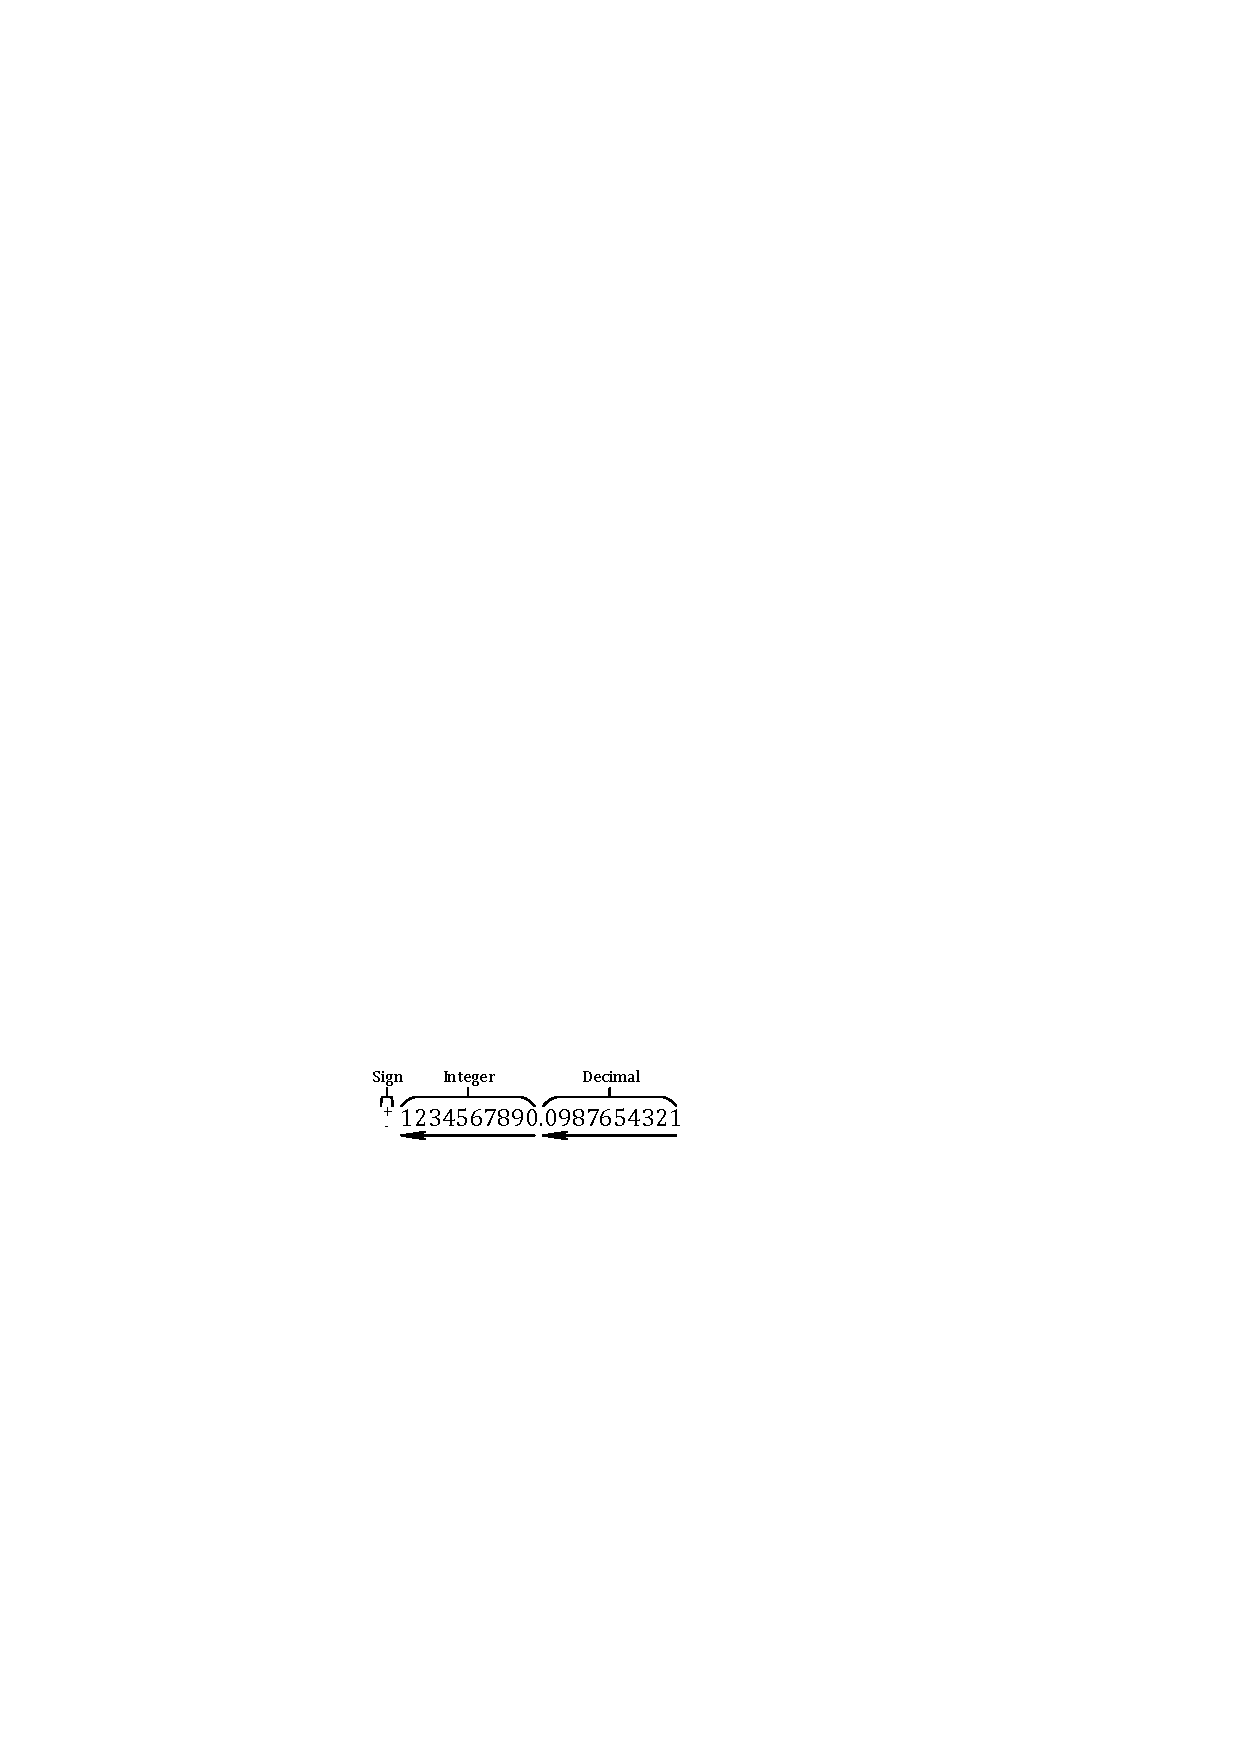
\includegraphics[scale=1.0]{./algorithm/real/pic/design/data_format_v3.pdf}
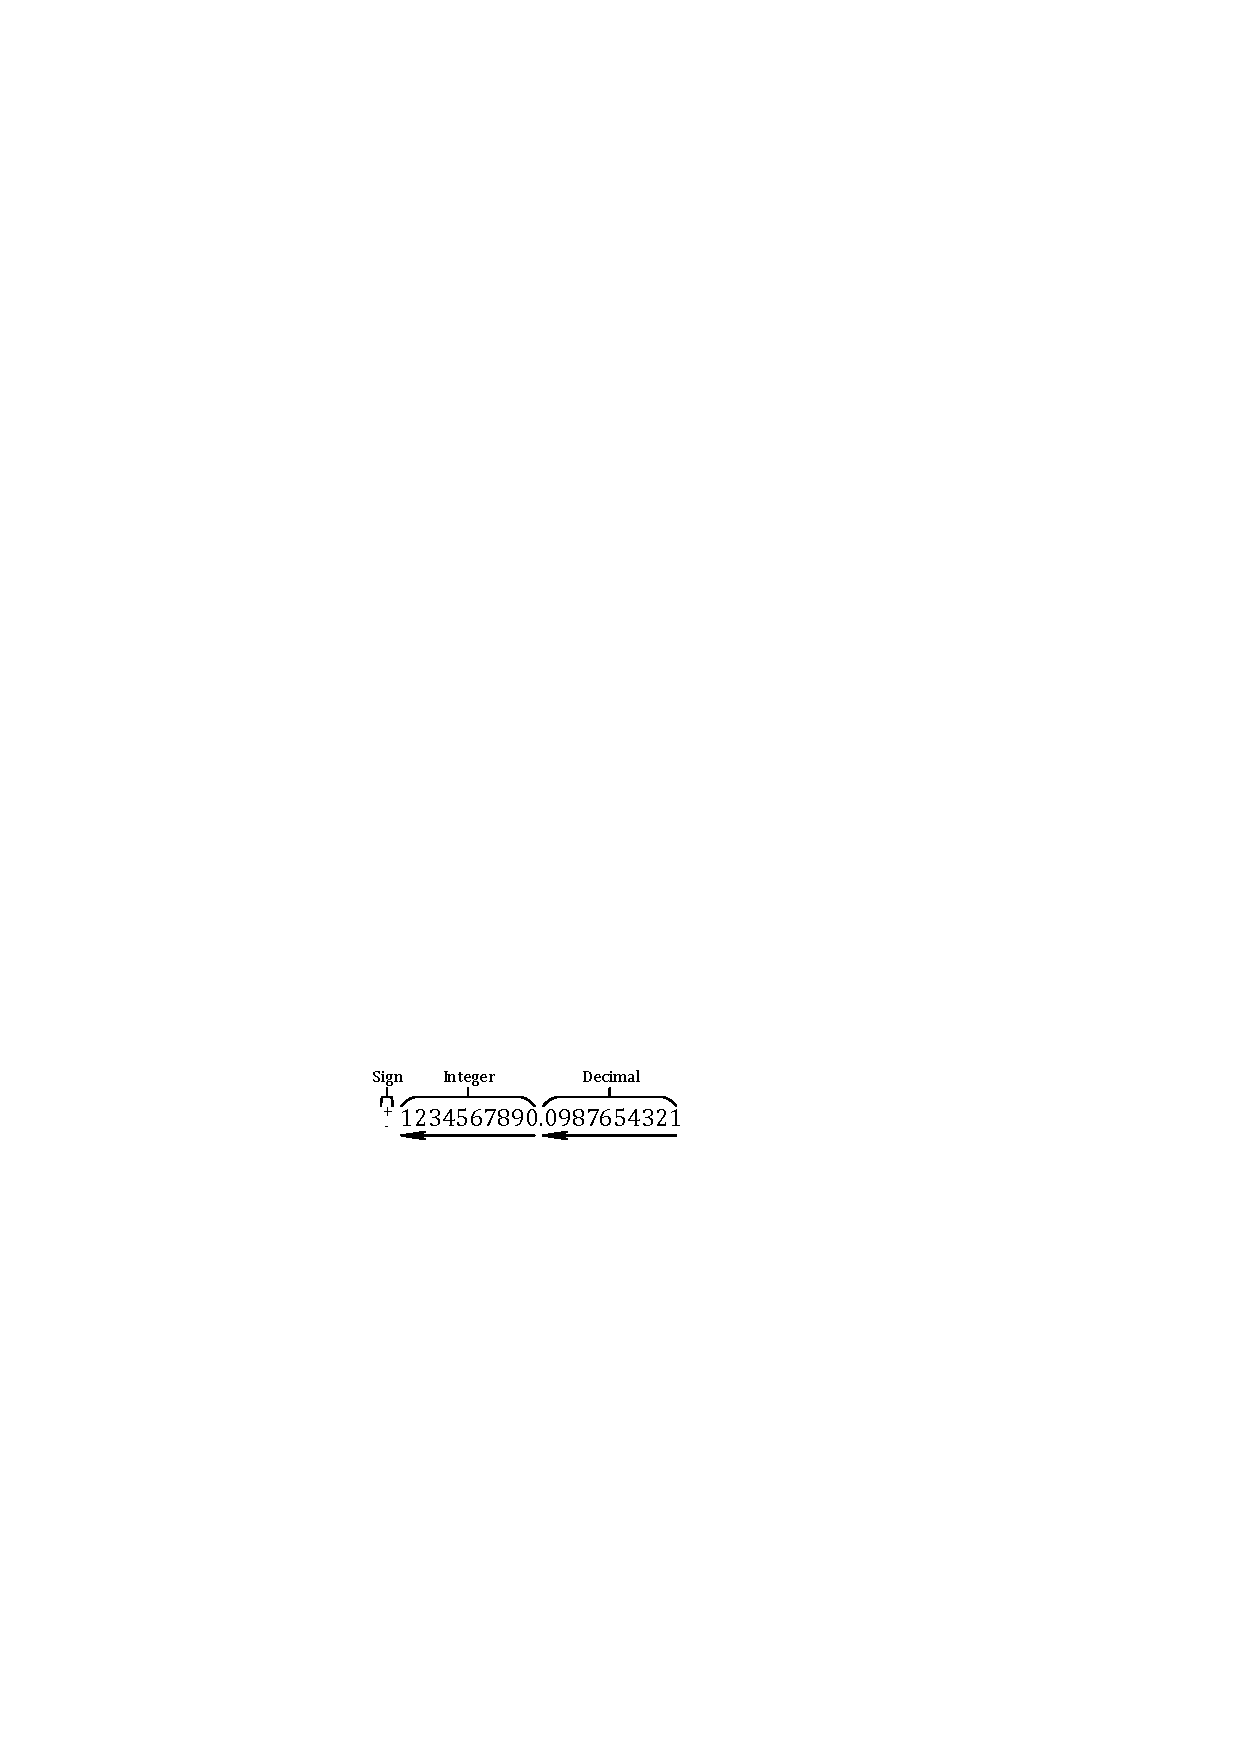
\includegraphics[width=0.6\textwidth]{./algorithm/real/pic/design/data_format_v3.pdf}
\caption{Data format of \textit{REAL} type.}
\label{fig:algorithm:real:data_format}
\end{figure}

The data format (figure \ref{fig:algorithm:real:data_format}) of \textit{REAL} is little bit different than the normal data concept, the value is as same as normal, the number at the left hand side means larger.\\

But when in the storage view is different, the \textit{"Integer"} part is store in normal and inverted order which will explain in the example of each operation, but the \textit{"Decimal"} part is using inverted which means the value will inverted when it stored. We use figure \ref{fig:algorithm:real:data_store_inverted} to explain why we do this.

\begin{figure}[h]
\centering
    \begin{subfigure}[b]{0.4\textwidth}
        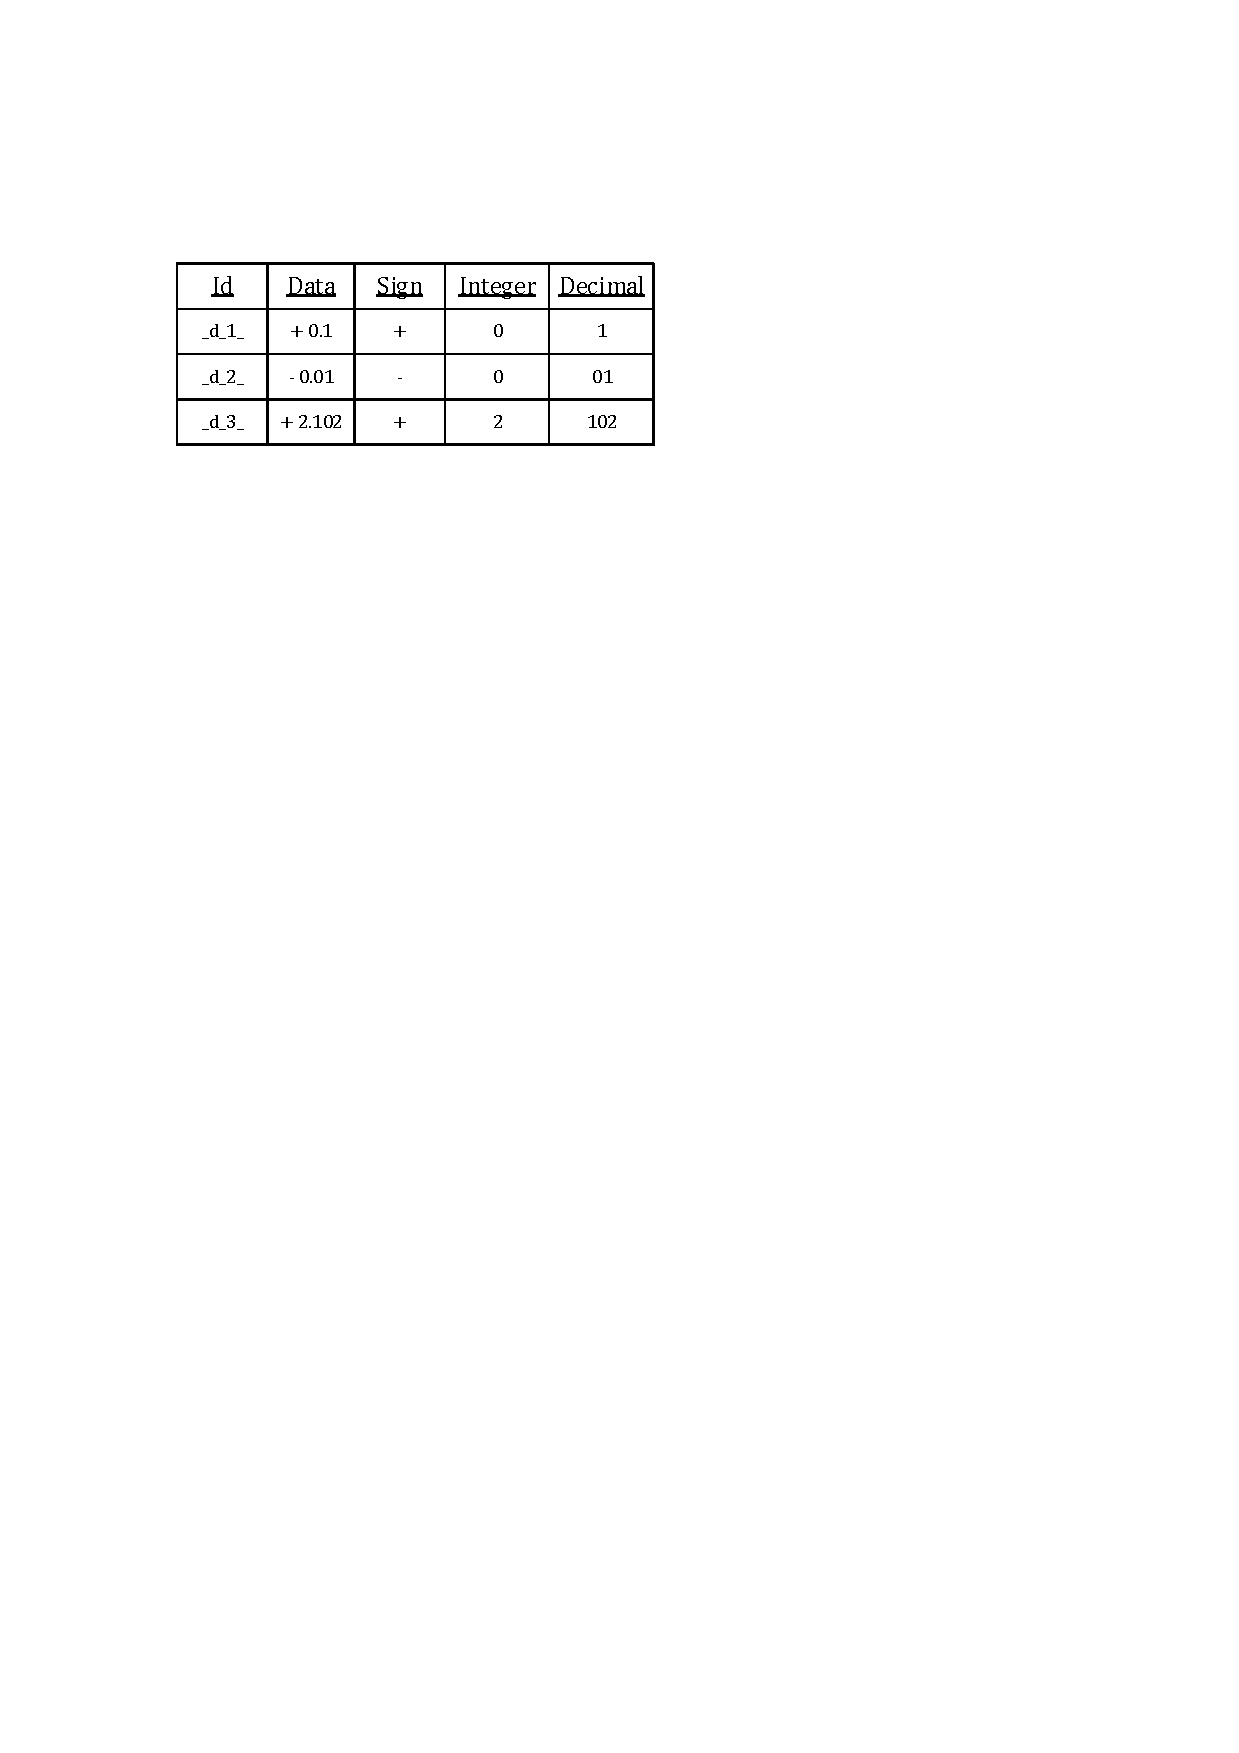
\includegraphics[width=\textwidth]{./algorithm/real/pic/design/data_store_inverted_1_v1.pdf}
        \caption{Normal order}
        \label{fig:algorithm:real:data_store_inverted_1}
    \end{subfigure}%
    ~ %add desired spacing between images, e. g. ~, \quad, \qquad etc.
          %(or a blank line to force the subfigure onto a new line)
    \begin{subfigure}[b]{0.4\textwidth}
        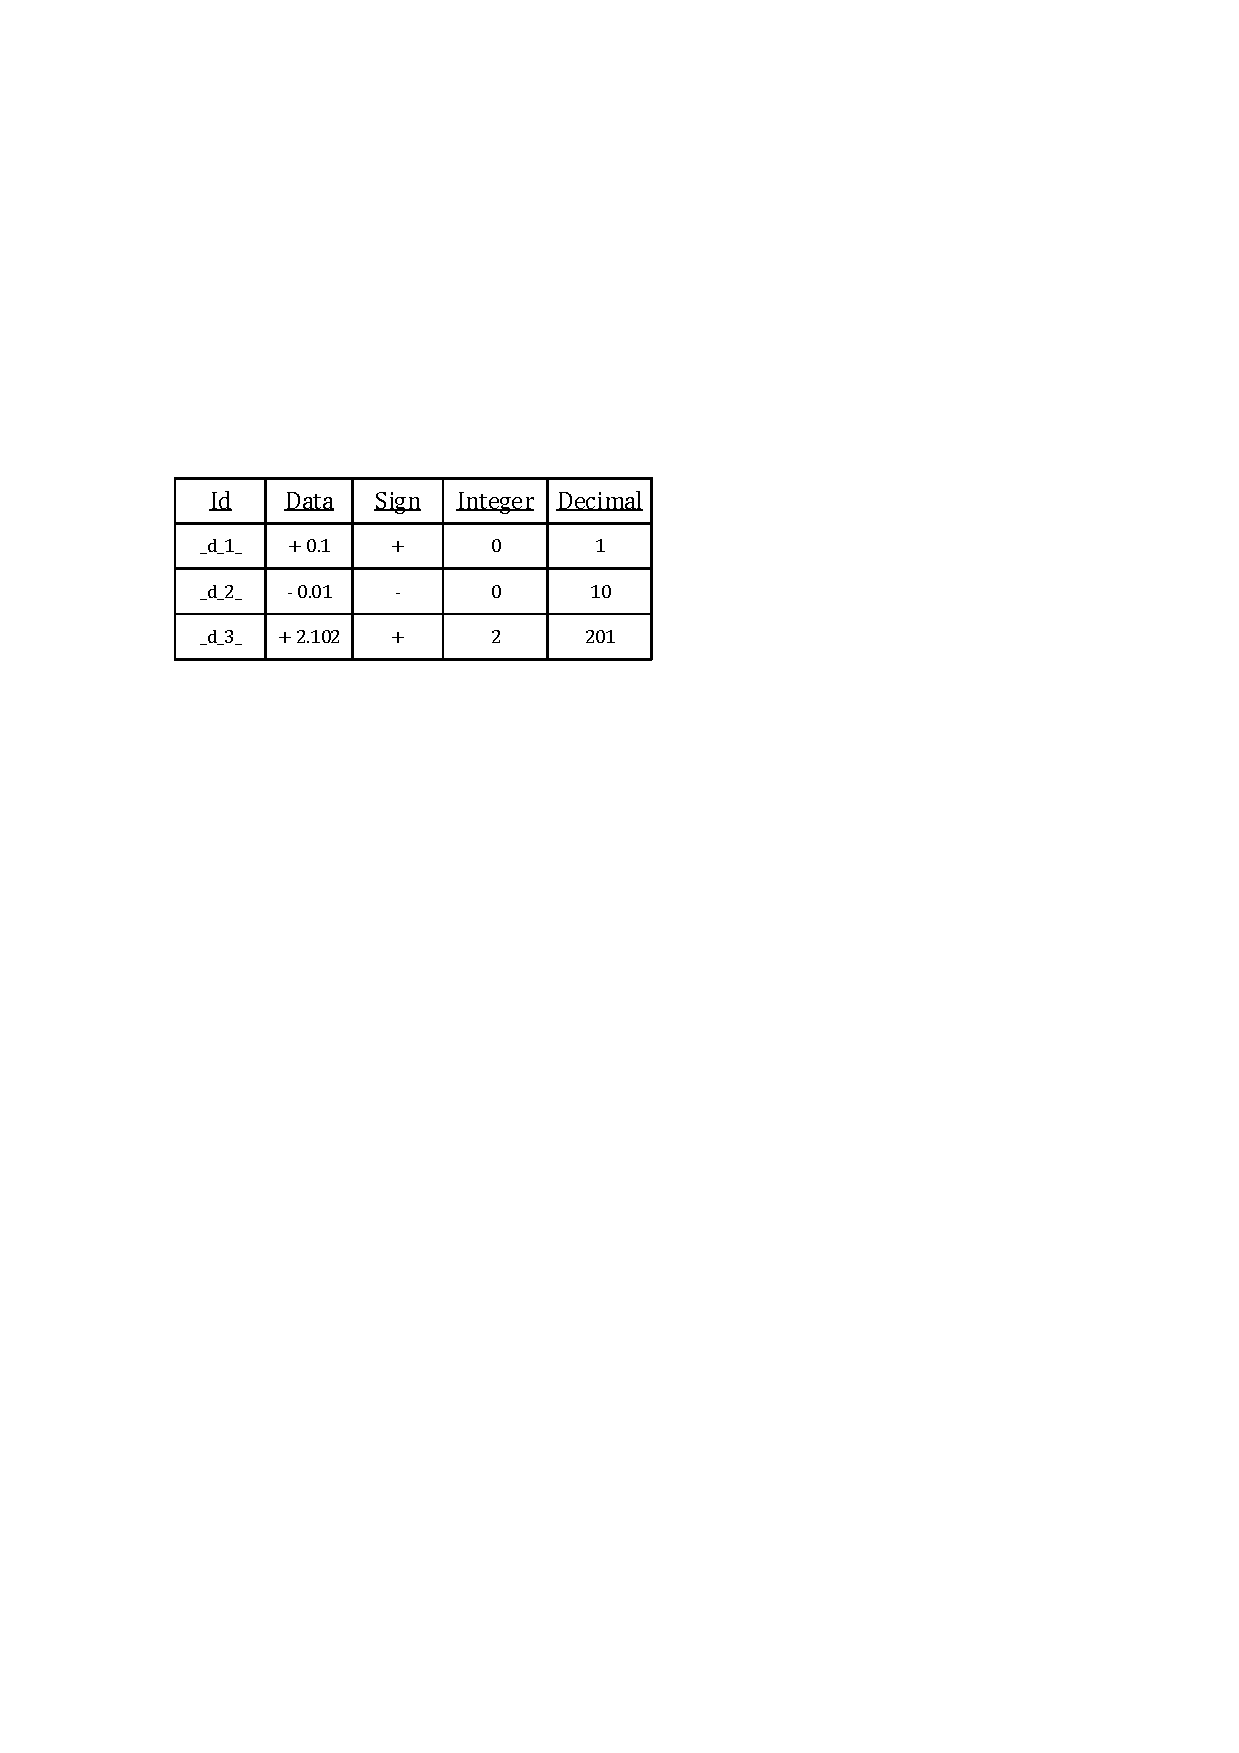
\includegraphics[width=\textwidth]{./algorithm/real/pic/design/data_store_inverted_2_v1.pdf}
        \caption{Inverted order}
        \label{fig:algorithm:real:data_store_inverted_2}
    \end{subfigure}

    \caption{Value storage}
    \label{fig:algorithm:real:data_store_inverted}
\end{figure}

If the data store as the same order as usual, the sample data will store like figure \ref{fig:algorithm:real:data_store_inverted_1}, the problem is if we treat \textit{'01'} as a value, it will convert into \textit{'1'} and lost its owns meaning, because \textit{'.1'} is not equal \textit{'.01'}. So if invert the \textit{"Decimal"} part, the value will look like figure \ref{fig:algorithm:real:data_store_inverted_2}. It shows the value can be store without missing value, the only is a additional convert operation is need to revert back into the real value when return data.\\

\begin{figure}[h]
\centering
%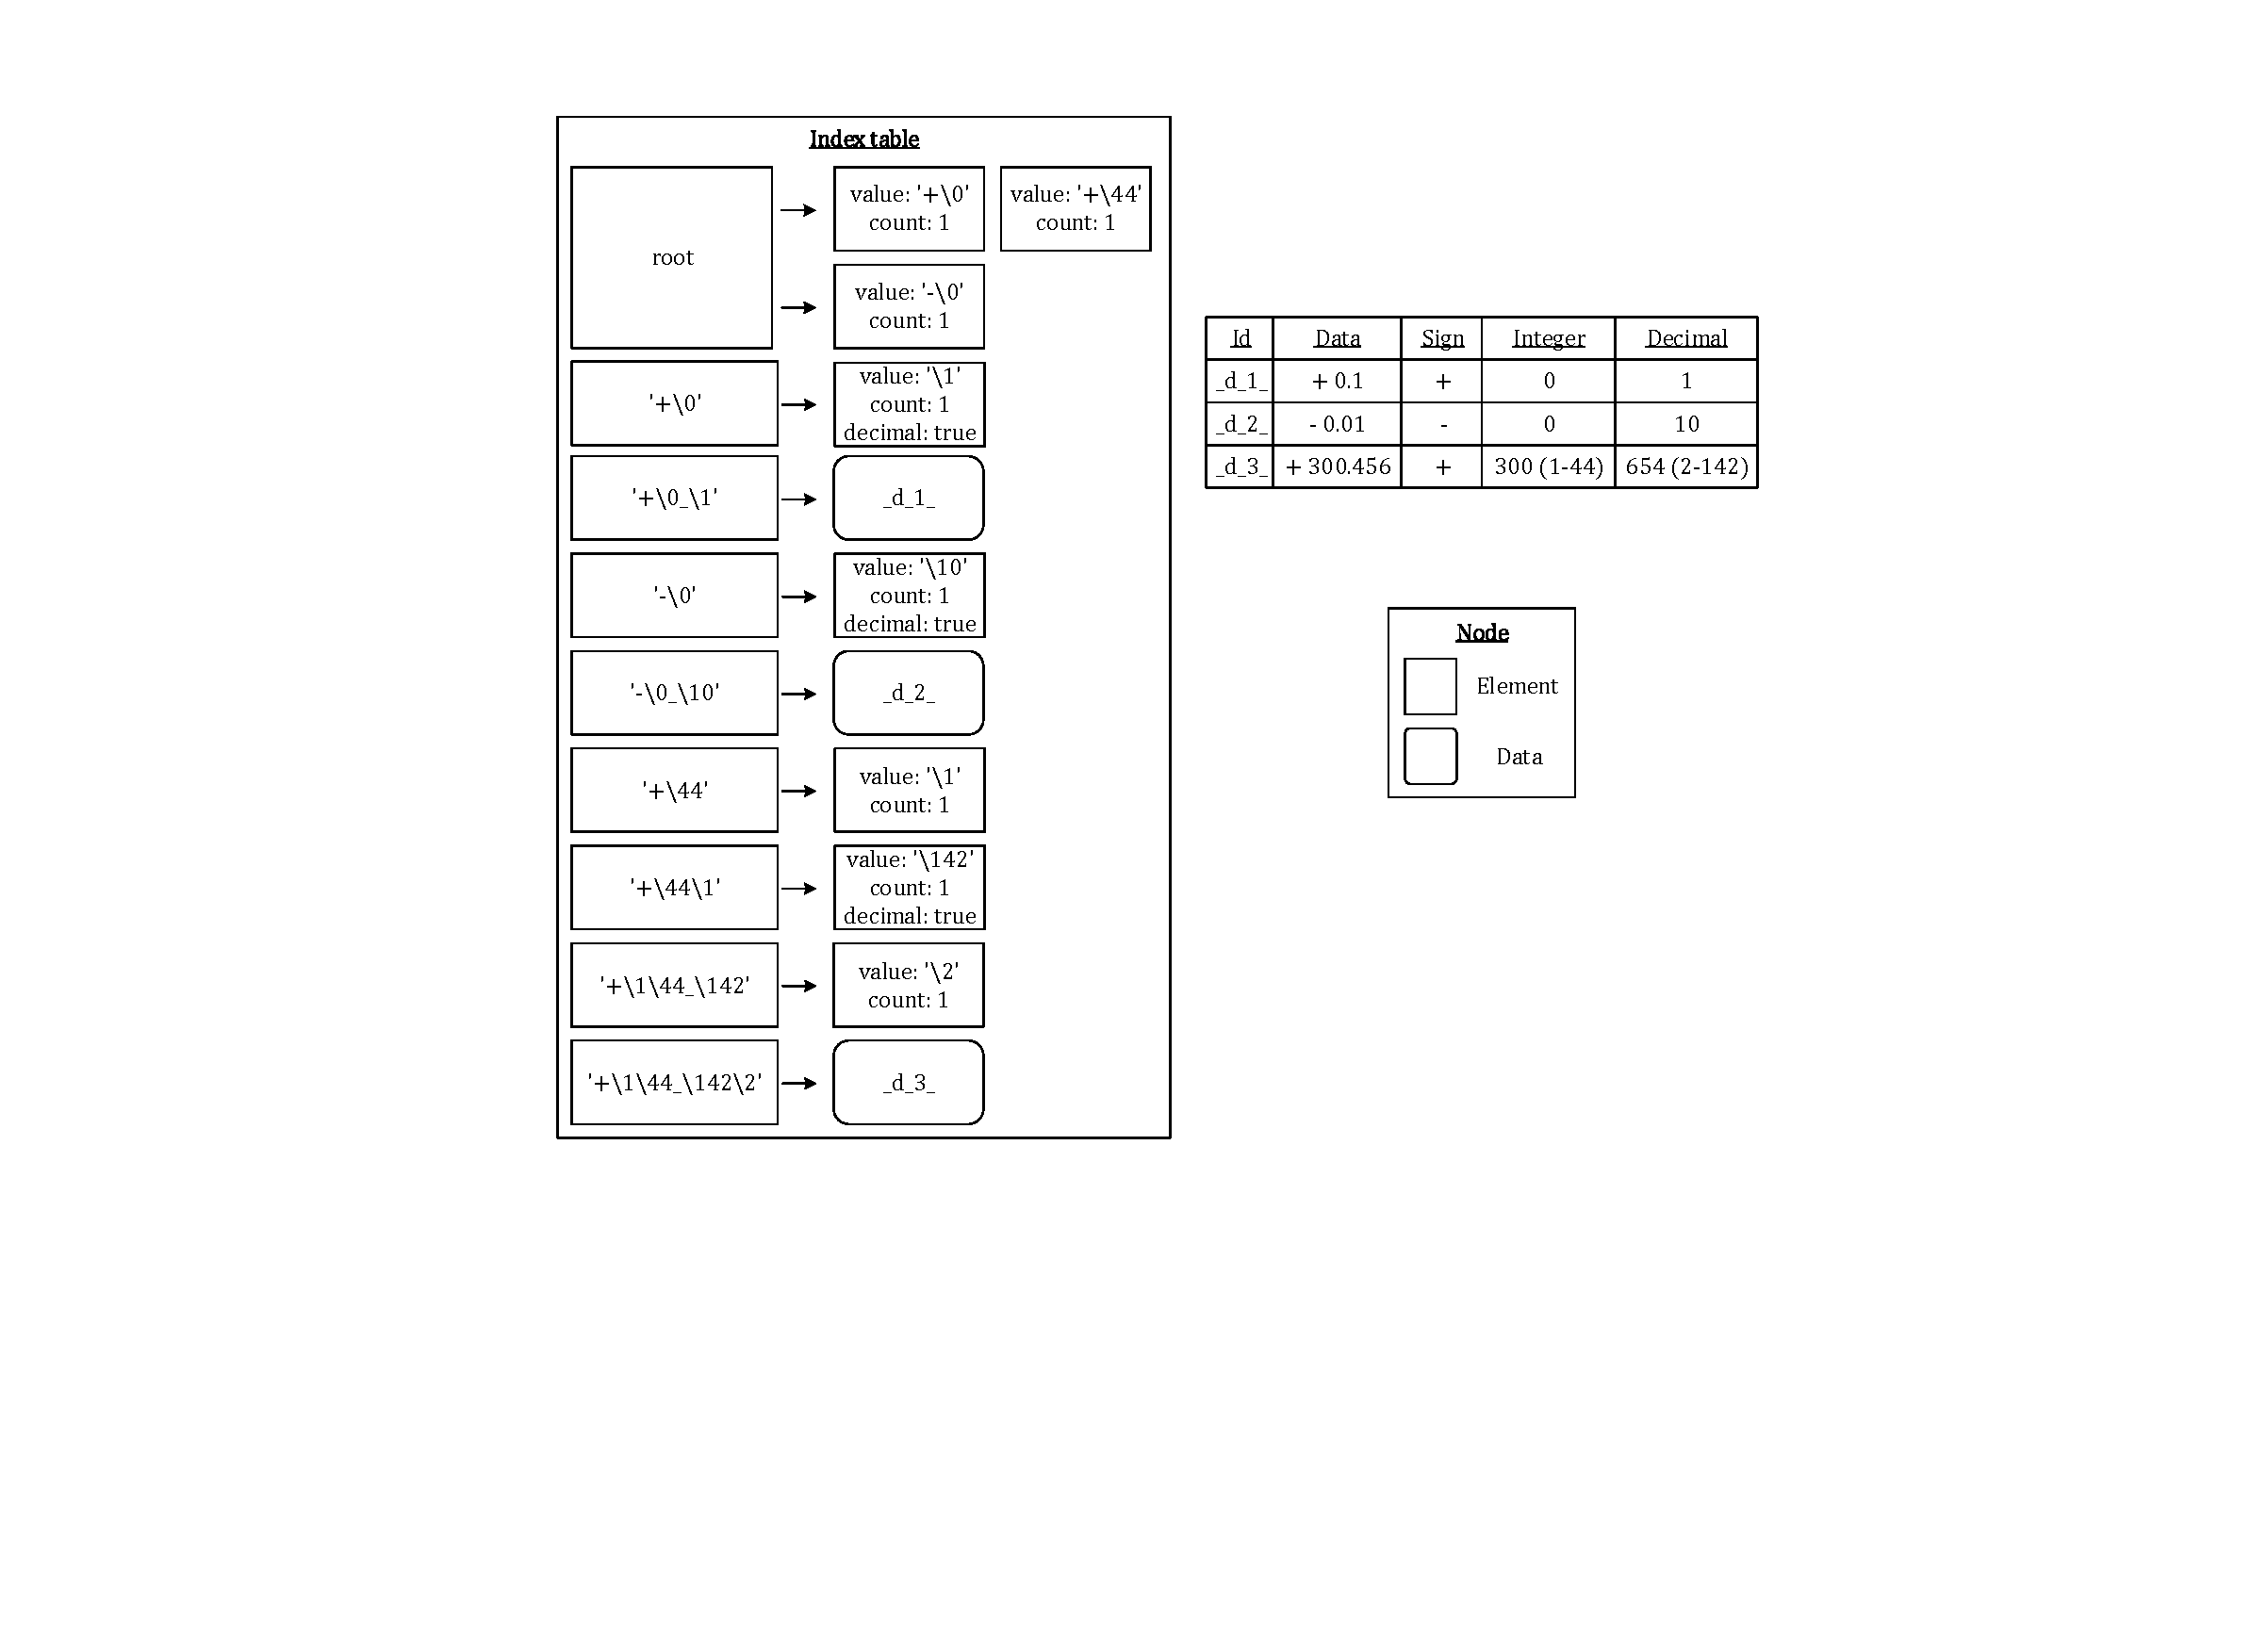
\includegraphics[scale=1.0]{./algorithm/real/pic/design/example_v4.pdf}
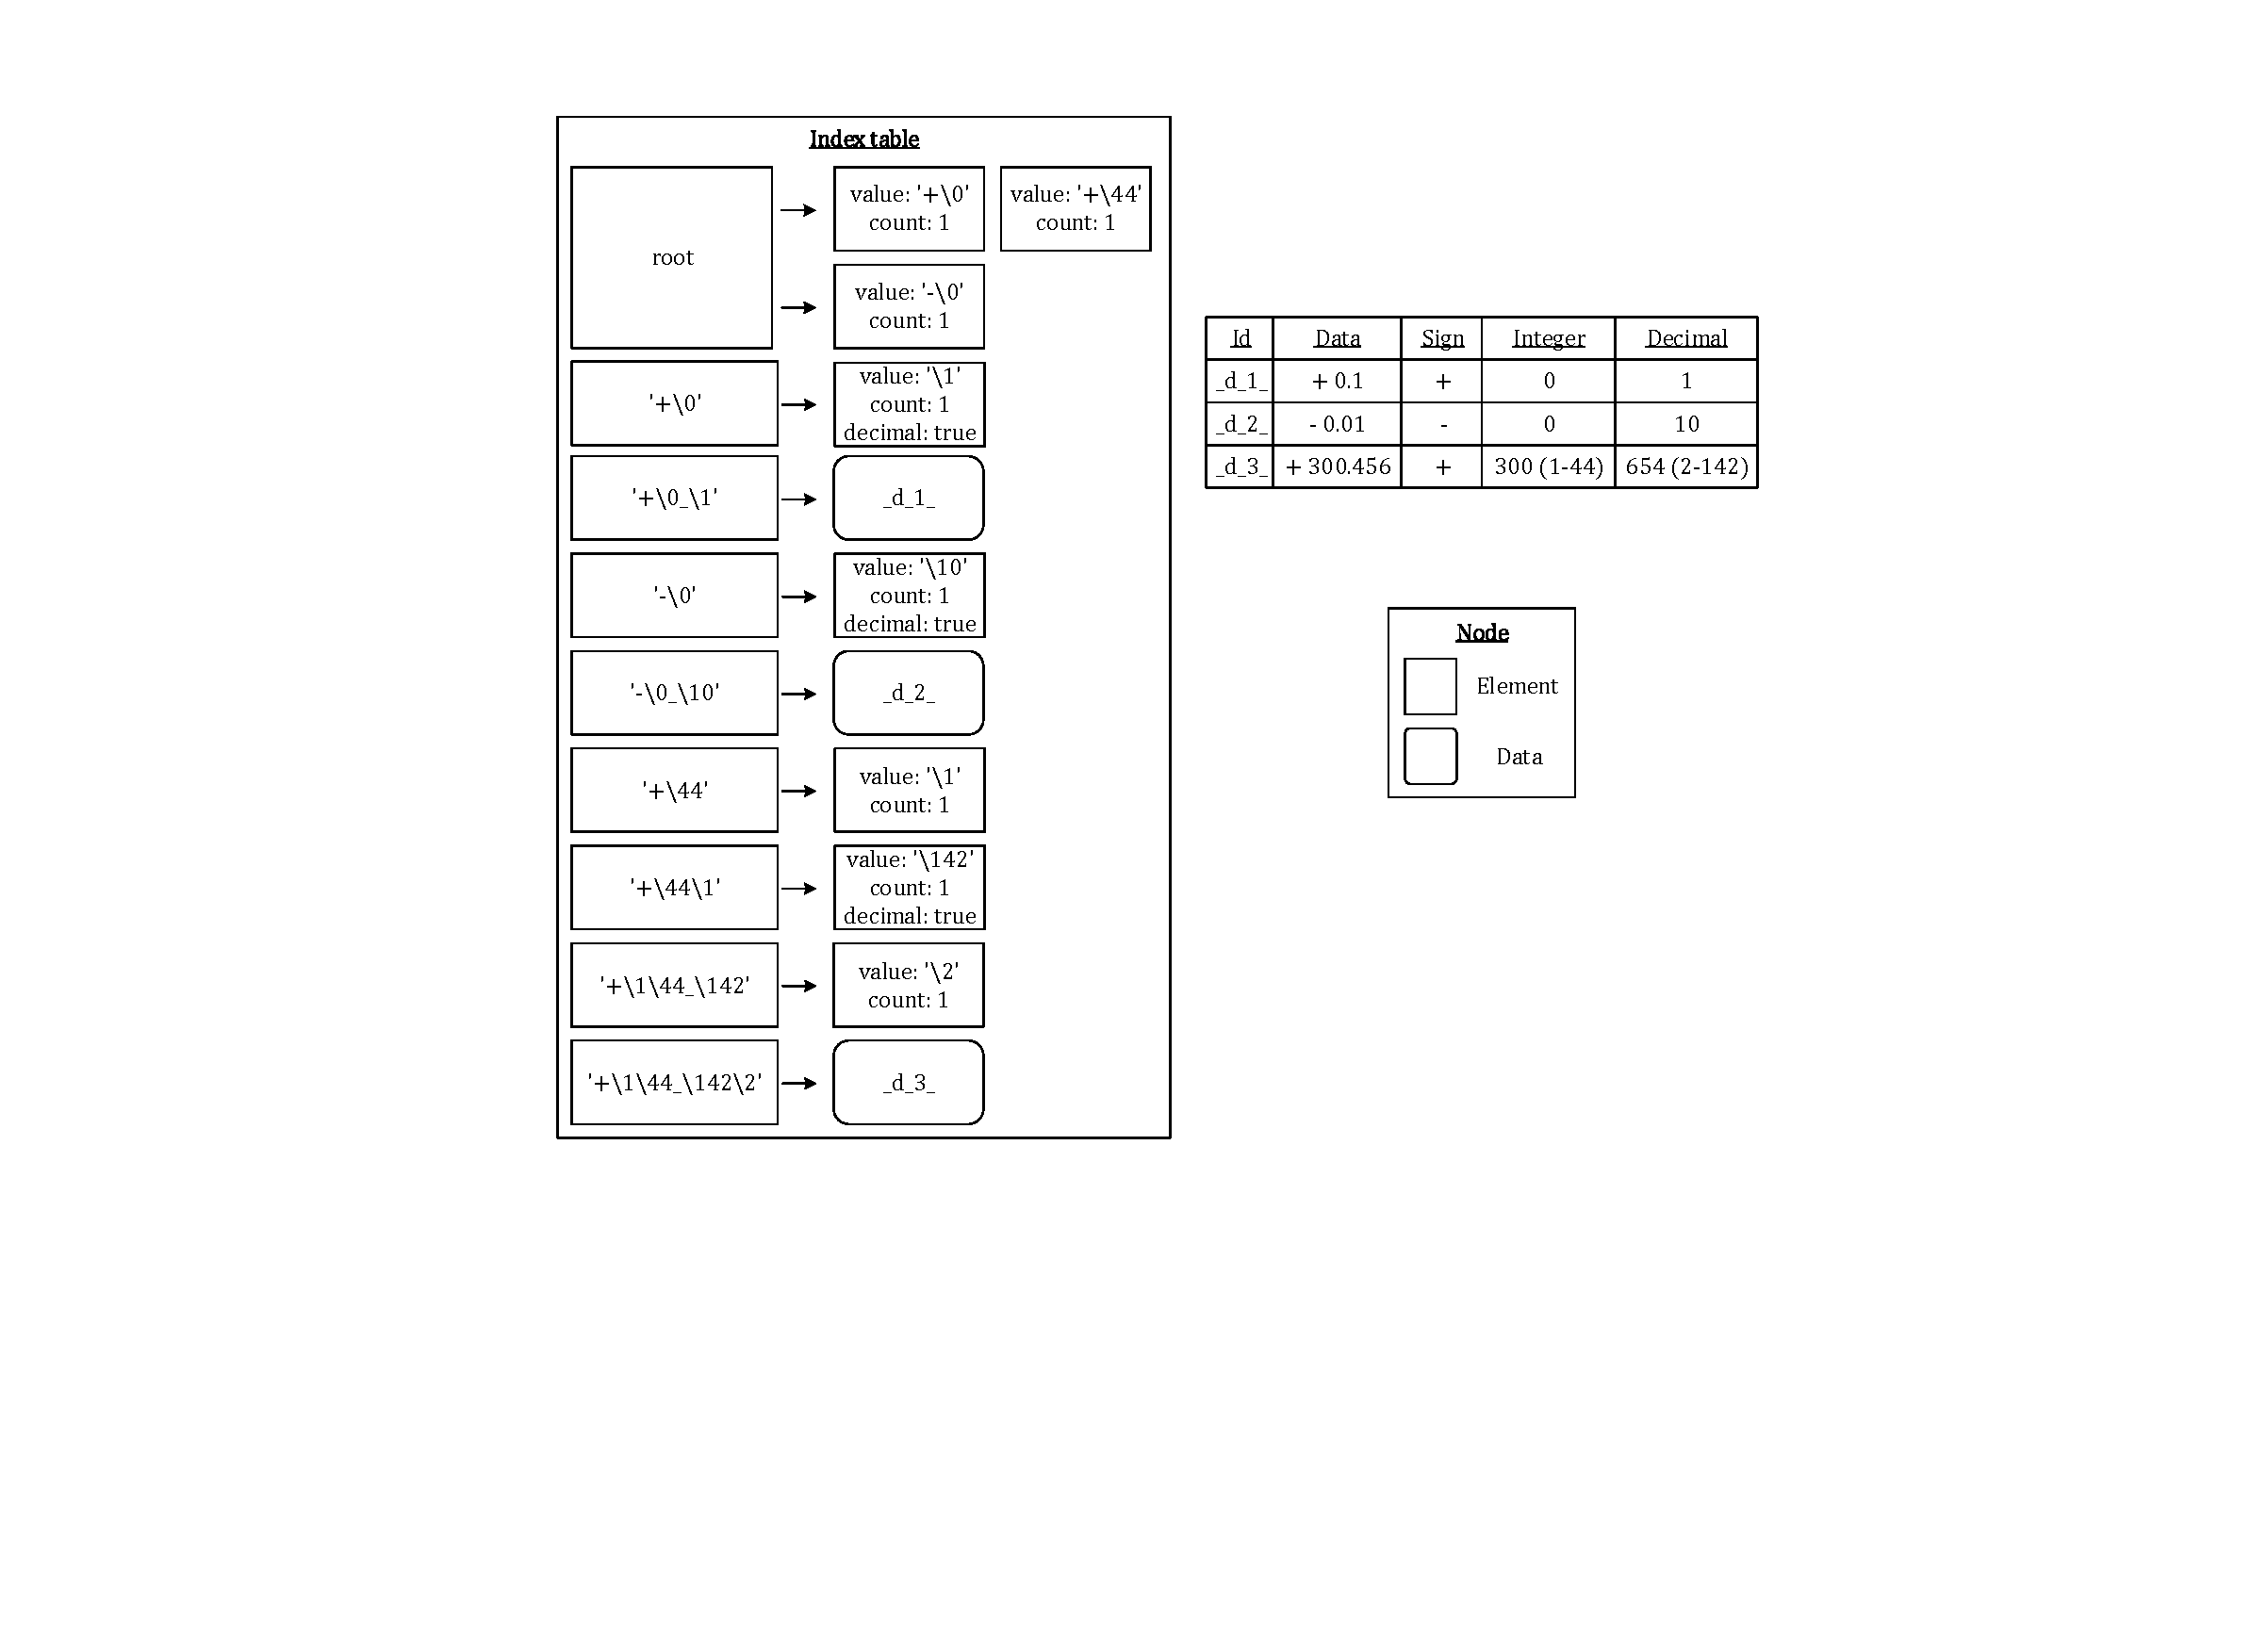
\includegraphics[width=0.8\textwidth]{./algorithm/real/pic/design/example_v4.pdf}
\caption{The index tables of \textit{REAL} type.}
\label{fig:algorithm:real:example}
\end{figure}

Figure \ref{fig:algorithm:real:example} is the example when storing data into index table. This table start with $root$ which is pointing to the \textit{"Sign"} part which is store with the last byte of \textit{"Integer"} part.

The \textit{"Integer"} is indexing using n-gram as normal, but it will index in two way:

\begin{enumerate}

\item When indexing the \textit{"Integer"} part only (like $'$+$\backslash44\backslash1'$ in figure), it is start from the last byte to the first, and then will pointing to the element node which contain a flag that means as $decimal$, which is represent to begin \textit{"Decimal"} part.

\item Like $'$+$\backslash1\backslash44\_\backslash2\backslash142'$ in figure, the order of the \textit{"Integer"} part is store as from the left to right when it is storing with the \textit{"Decimal"} part.

\end{enumerate}

And \textit{"Decimal"} is store from right to left, and because the inverted string value design which means if the value is small then it will become a greater value.

This order of \textit{"Integer"} and \textit{"Decimal"} part design is because this can do faster searching the key when doing sorting and comparison, this will explan detail in fellowing section.

% Insertion section
\subsubsection{Insertion}

In description and figure \ref{fig:algorithm:real:example} have already mentioned some of the flow of insertion, so in here will show the table if insert another value into the table. Insert $\pi (3.14159)$ into table, which will become like figure \ref{fig:algorithm:real:insertion:example}.

\begin{figure}[h]
\centering
%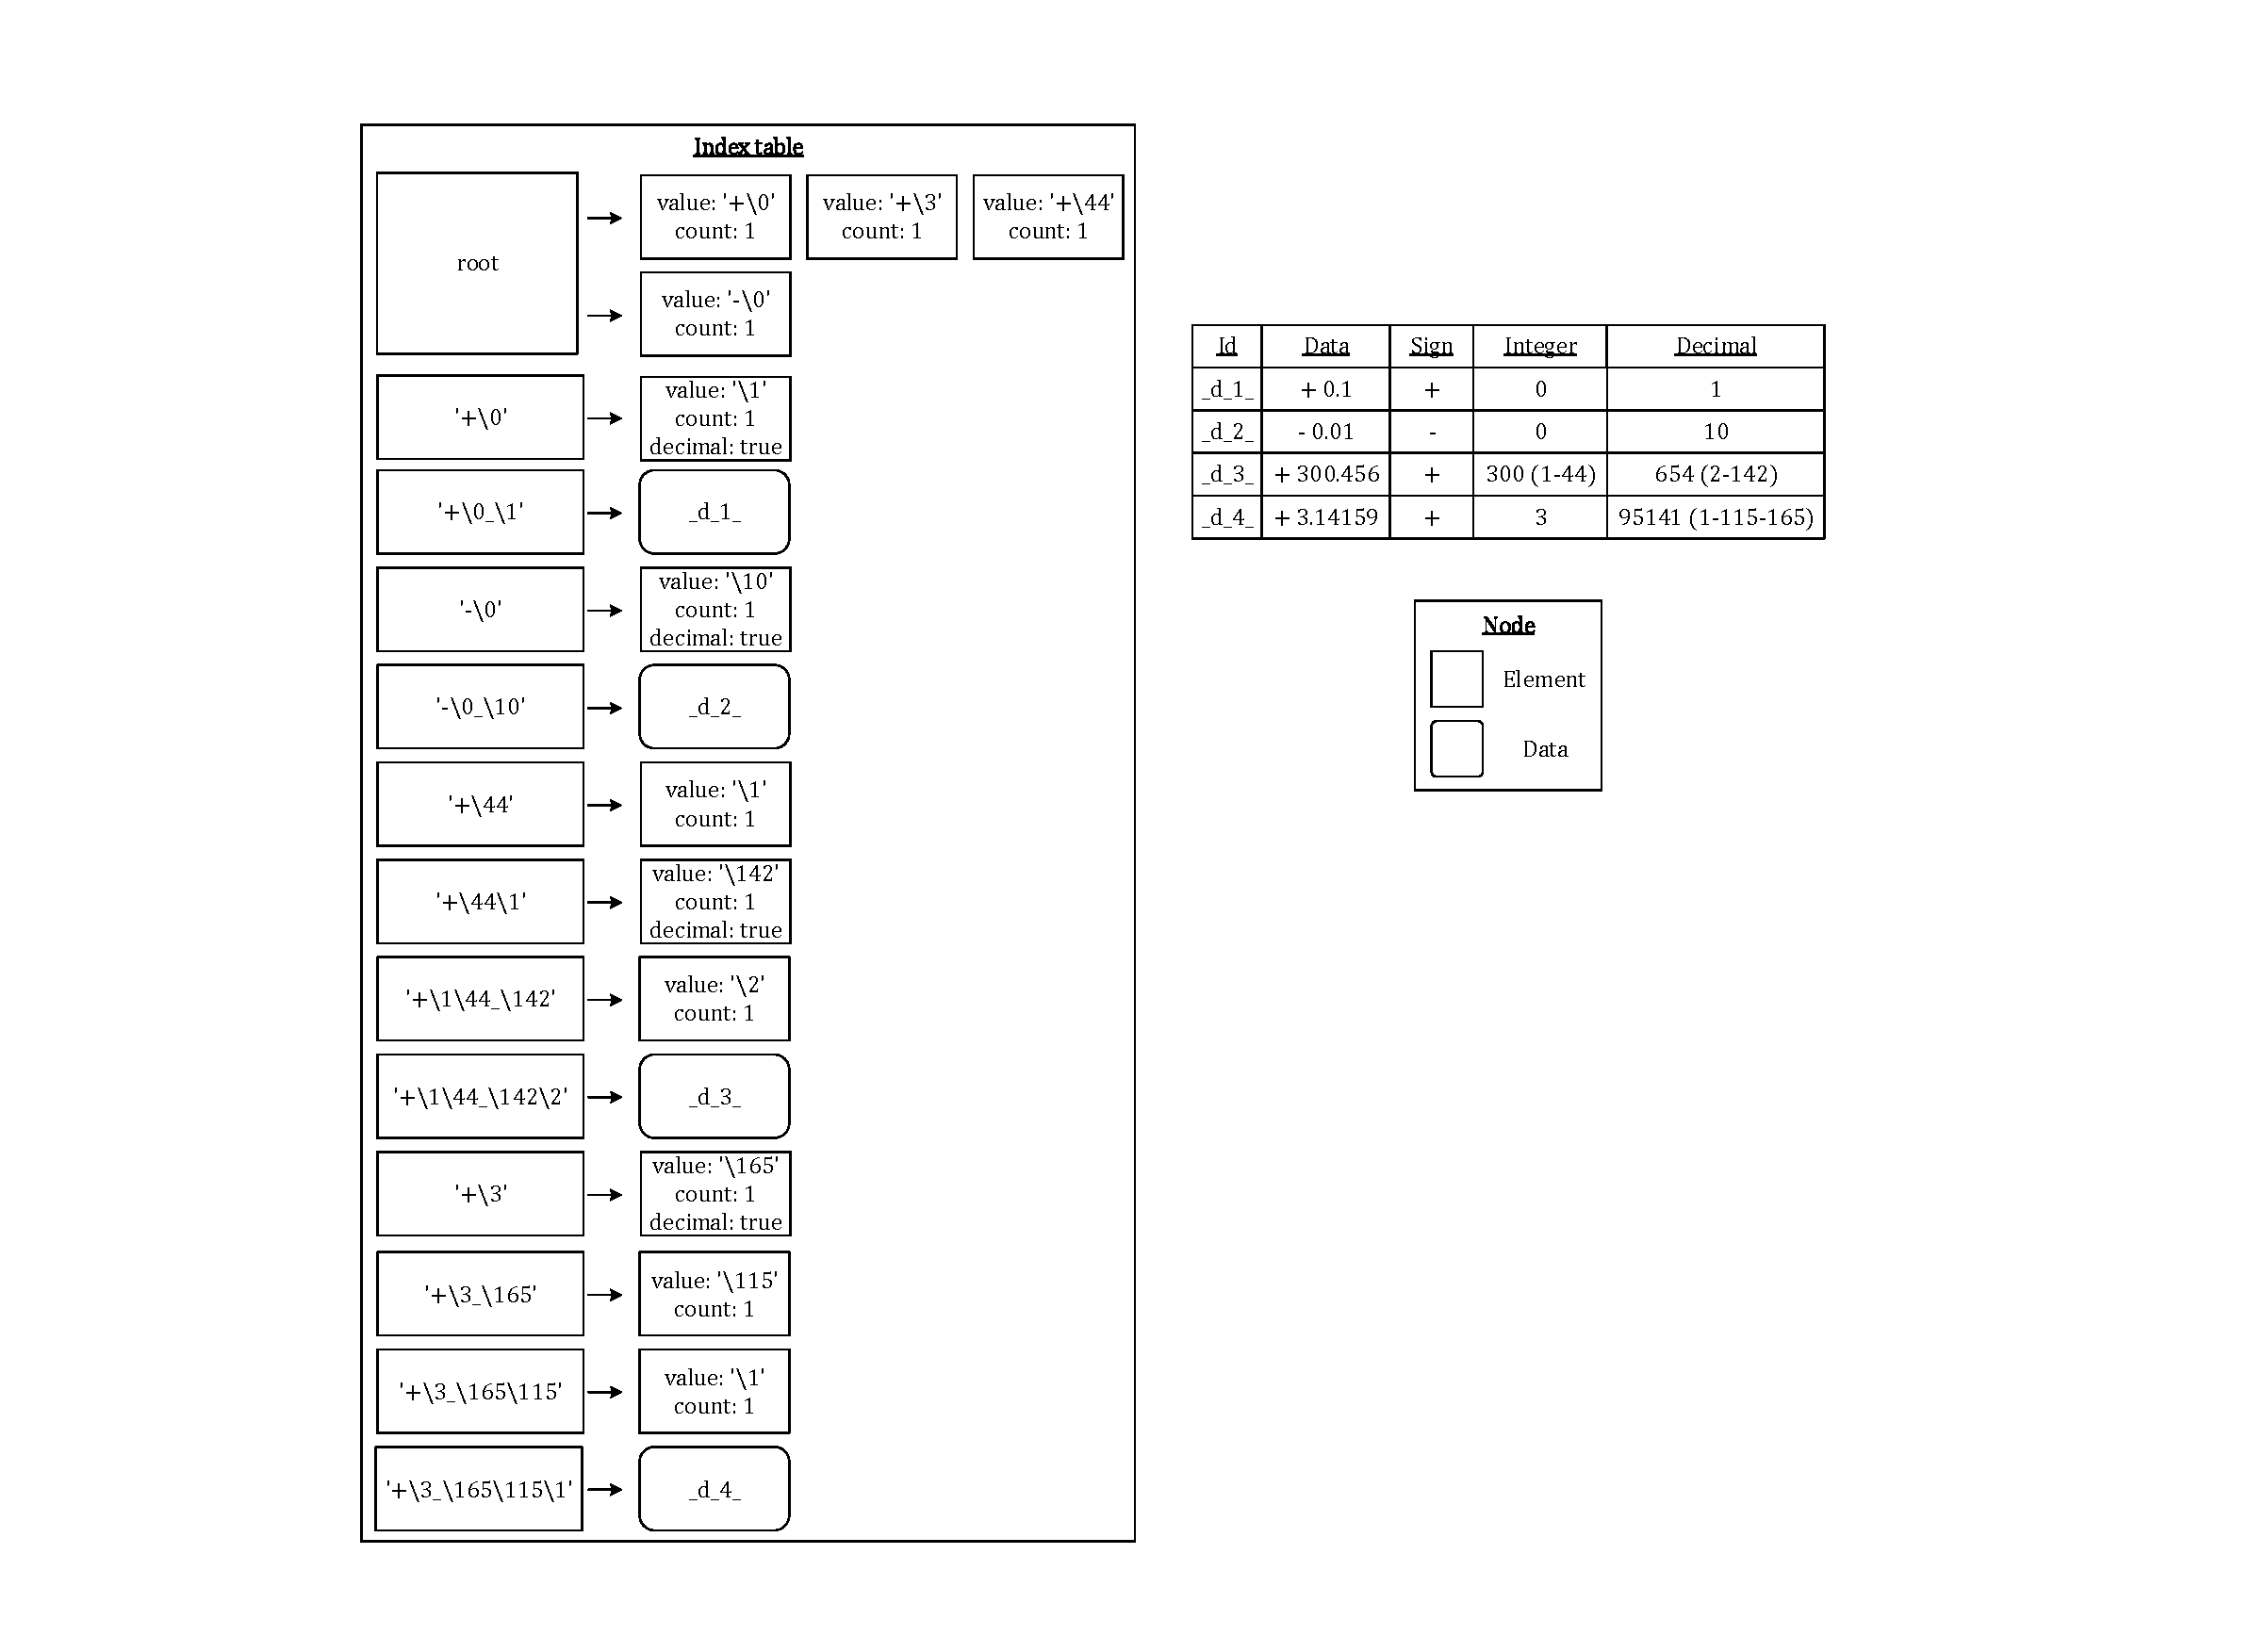
\includegraphics[scale=0.45]{./algorithm/real/pic/insertion/example_v4.png}
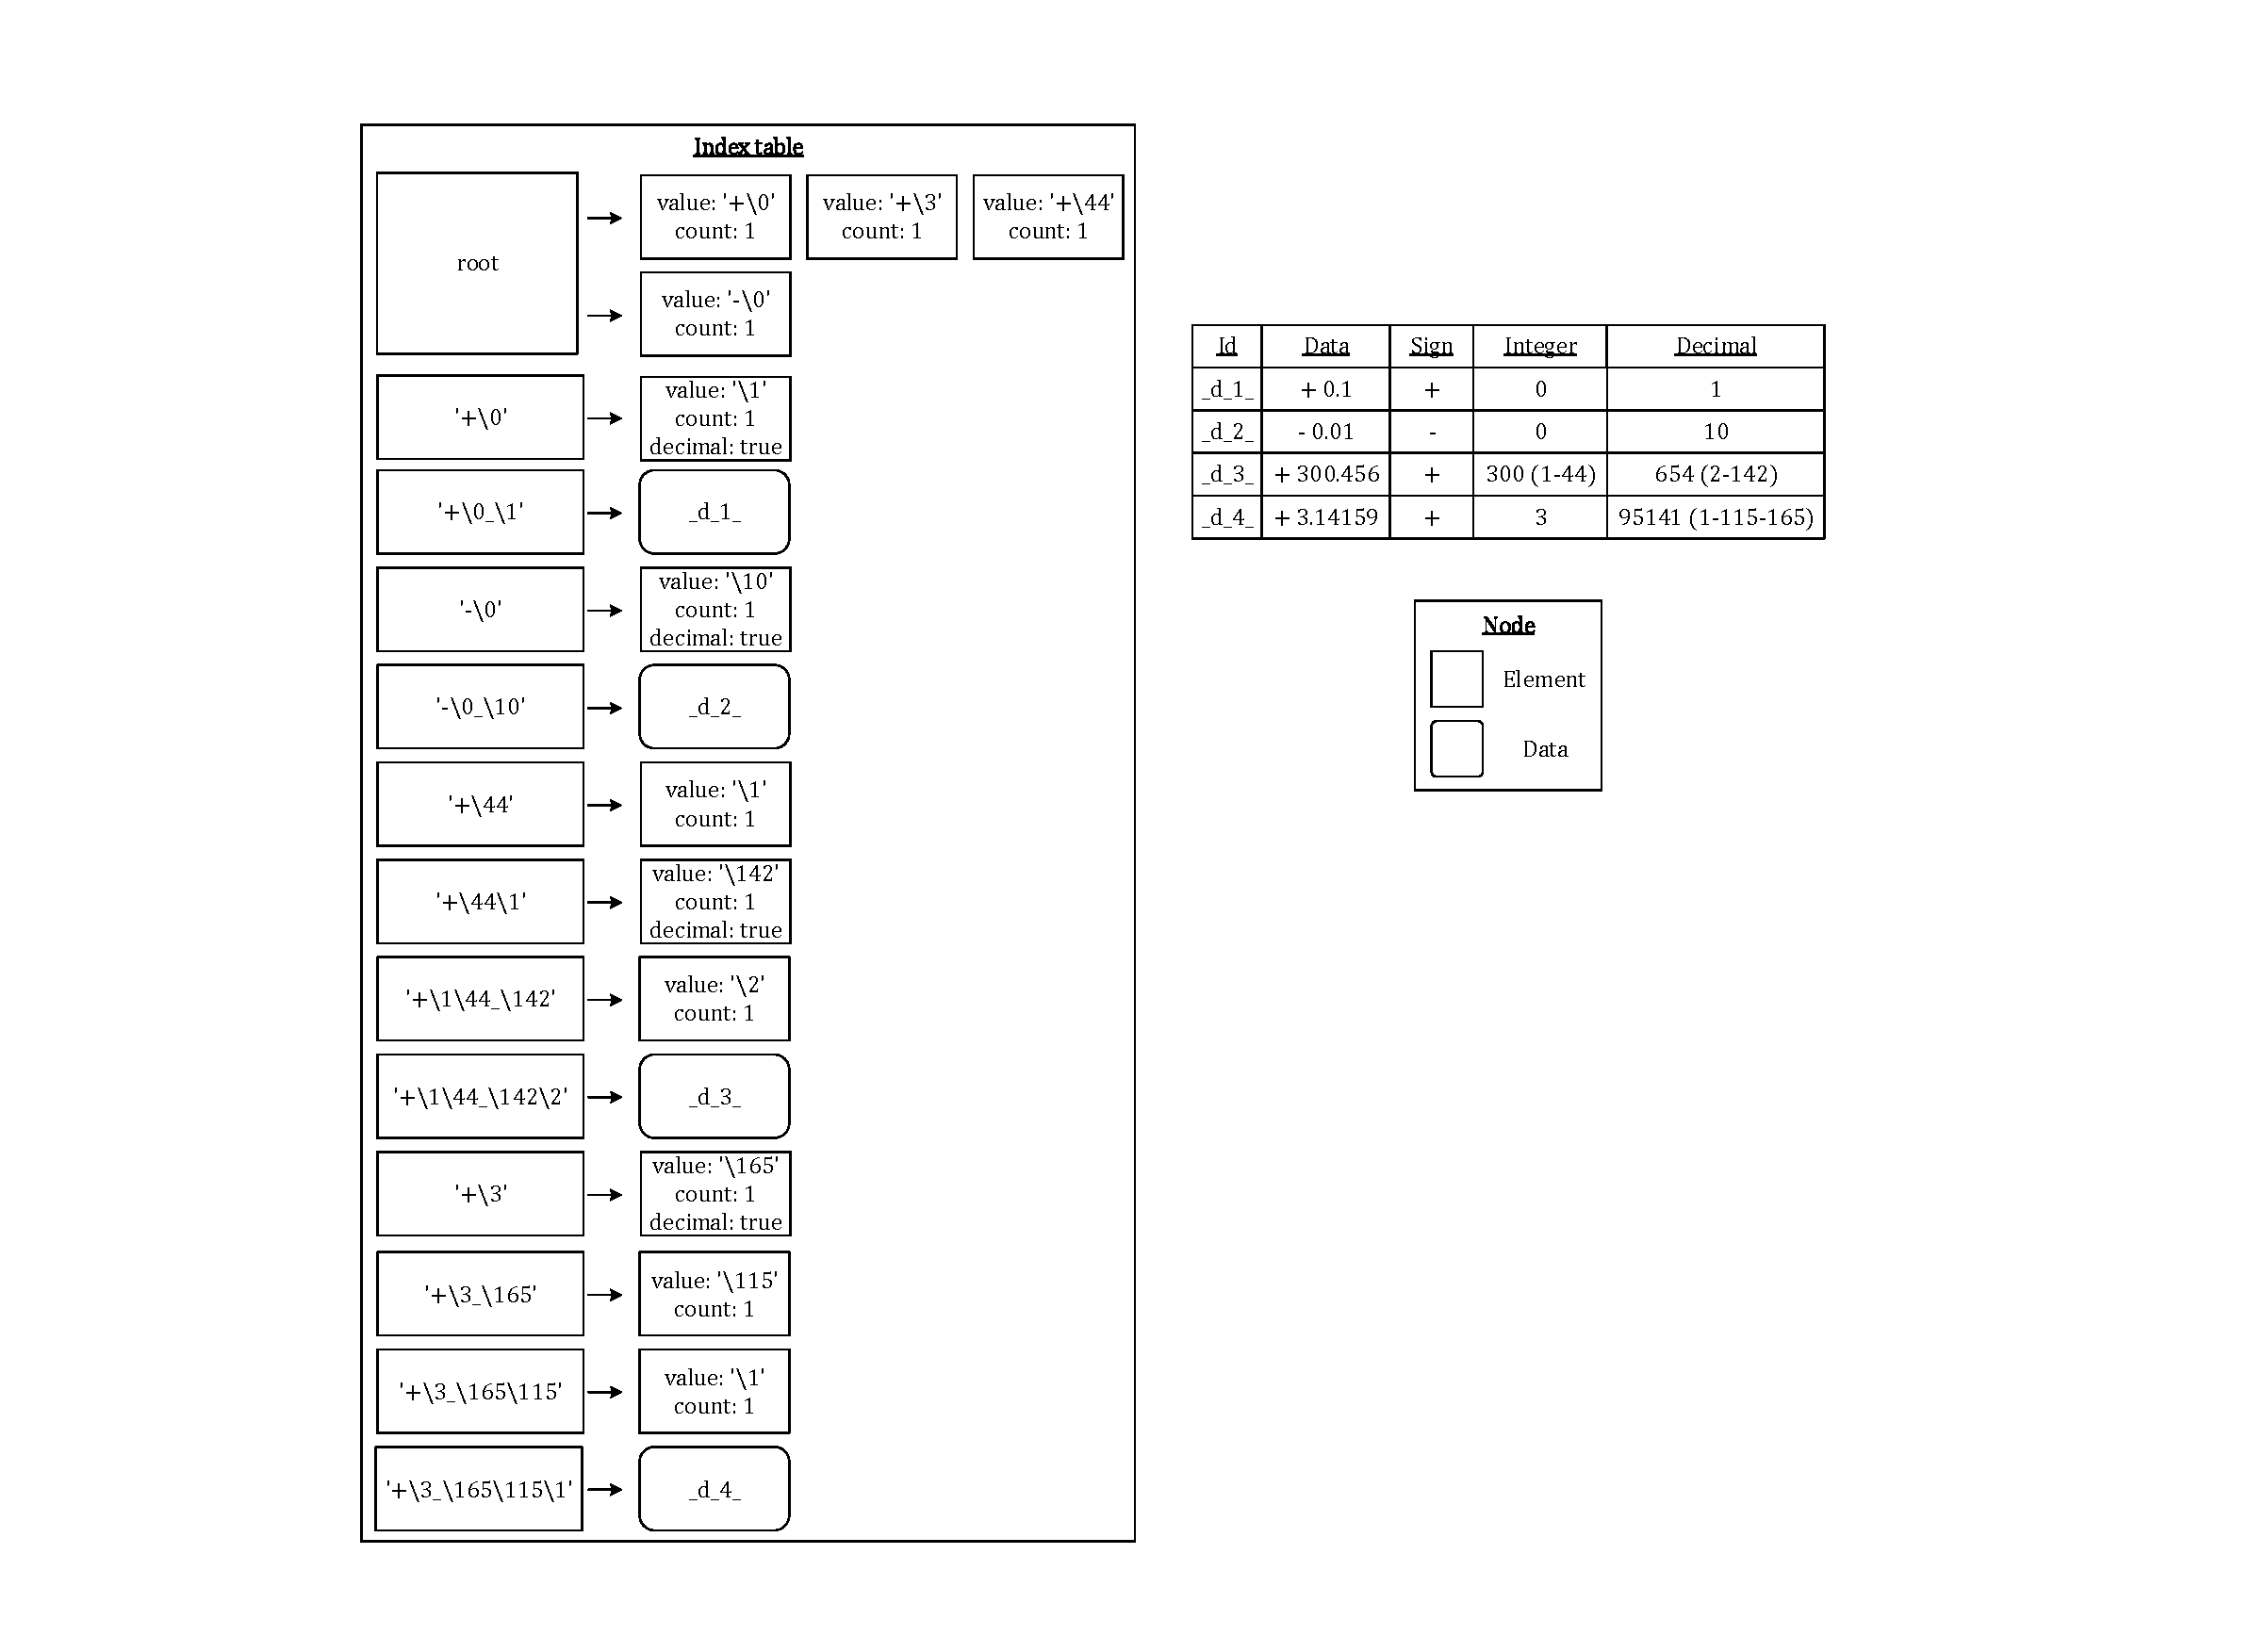
\includegraphics[width=0.8\textwidth]{./algorithm/real/pic/insertion/example_v4.pdf}
\caption{The table after inserted $\pi (3.14159)$.}
\label{fig:algorithm:real:insertion:example}
\end{figure}

Figure \ref{fig:algorithm:real:insertion:example} shows that the $\pi (+3.14159)$ is store the value by its \textit{"Sign"} $(+)$, \textit{"Integer"} $(3)$ and \textit{"Decimal"} $(95141)$.

The \textit{"Sign"} is pointing the last byte of the \textit{"Integer"}, the reason of point to the last byte is because of the dynamic length of \textit{REAL}, also assume the the byte of the data is longer than the input byte length:

\begin{enumerate}

\item  If the \textit{"Sign"} is pointing the first byte, then when we search the result for the input, this may need to compare more byte or we need to get the whole \textit{"Integer"} in the worst case to sure that this value is suitable or not to the input.

\item If \textit{"Sign"} is pointing the last byte, then we just need to compare few bytes or the same byte length of the input that we can immediately to know that is a result or not. So this indexing can speed up the searching.

\end{enumerate}

Time complexity should be $O(b!)$ which domain as $O(b)$, and $b$ is the length of the byte needed where $b = 4$ in this case.



% Deletion section
\subsubsection{Deletion}

Deletion is just do the opposite insertion to remove the byte and decrease the count. So time complexity be $O(b)$.



% Modification section
\subsubsection{Modification}

The modify flow are similar as \textit{INTEGER} type, remove the key which don't needed and add the count if the byte is the same. So follow the example in figure \ref{fig:algorithm:real:insertion:example} and then modify -$0.01$ to +$0.0$ (because zero don't contain positive or negative sign, so using positive sign should be fine), the table will look like figure \ref{fig:algorithm:real:modification:example} and the time complexity be $O(b)$.

\begin{figure}[h]
\centering
%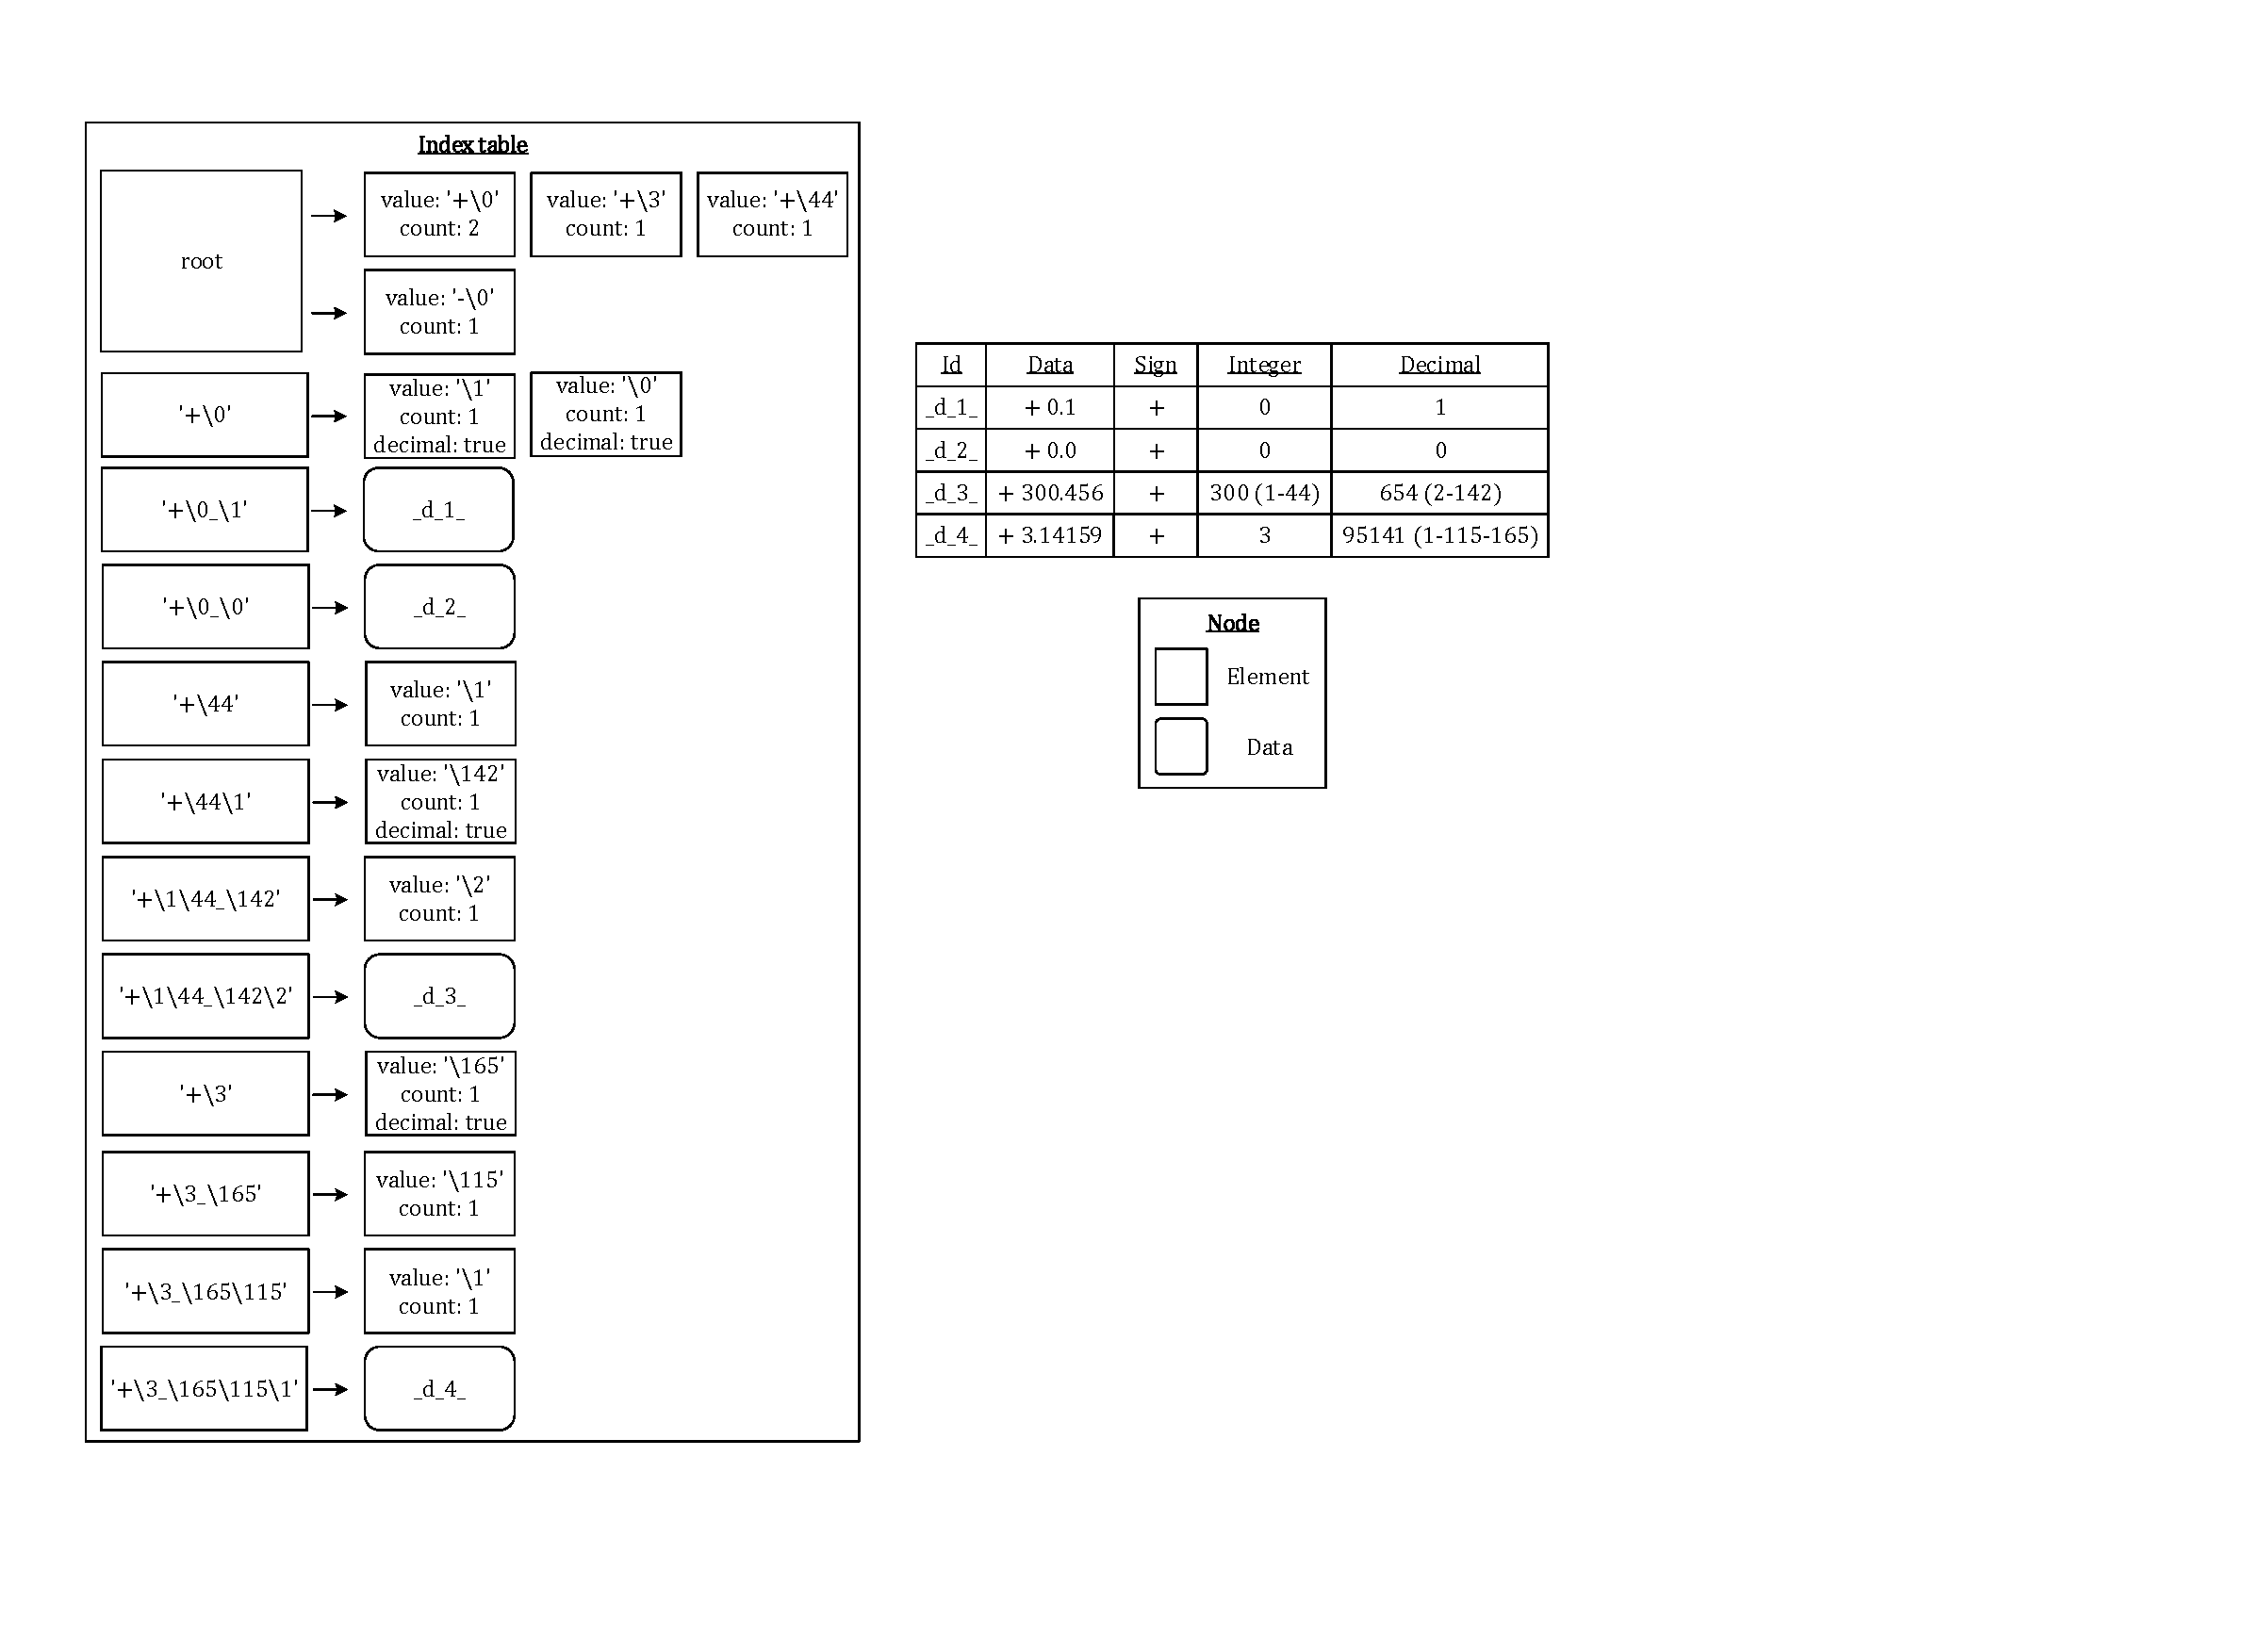
\includegraphics[scale=0.5]{./algorithm/real/pic/modification/example_v4.pdf}
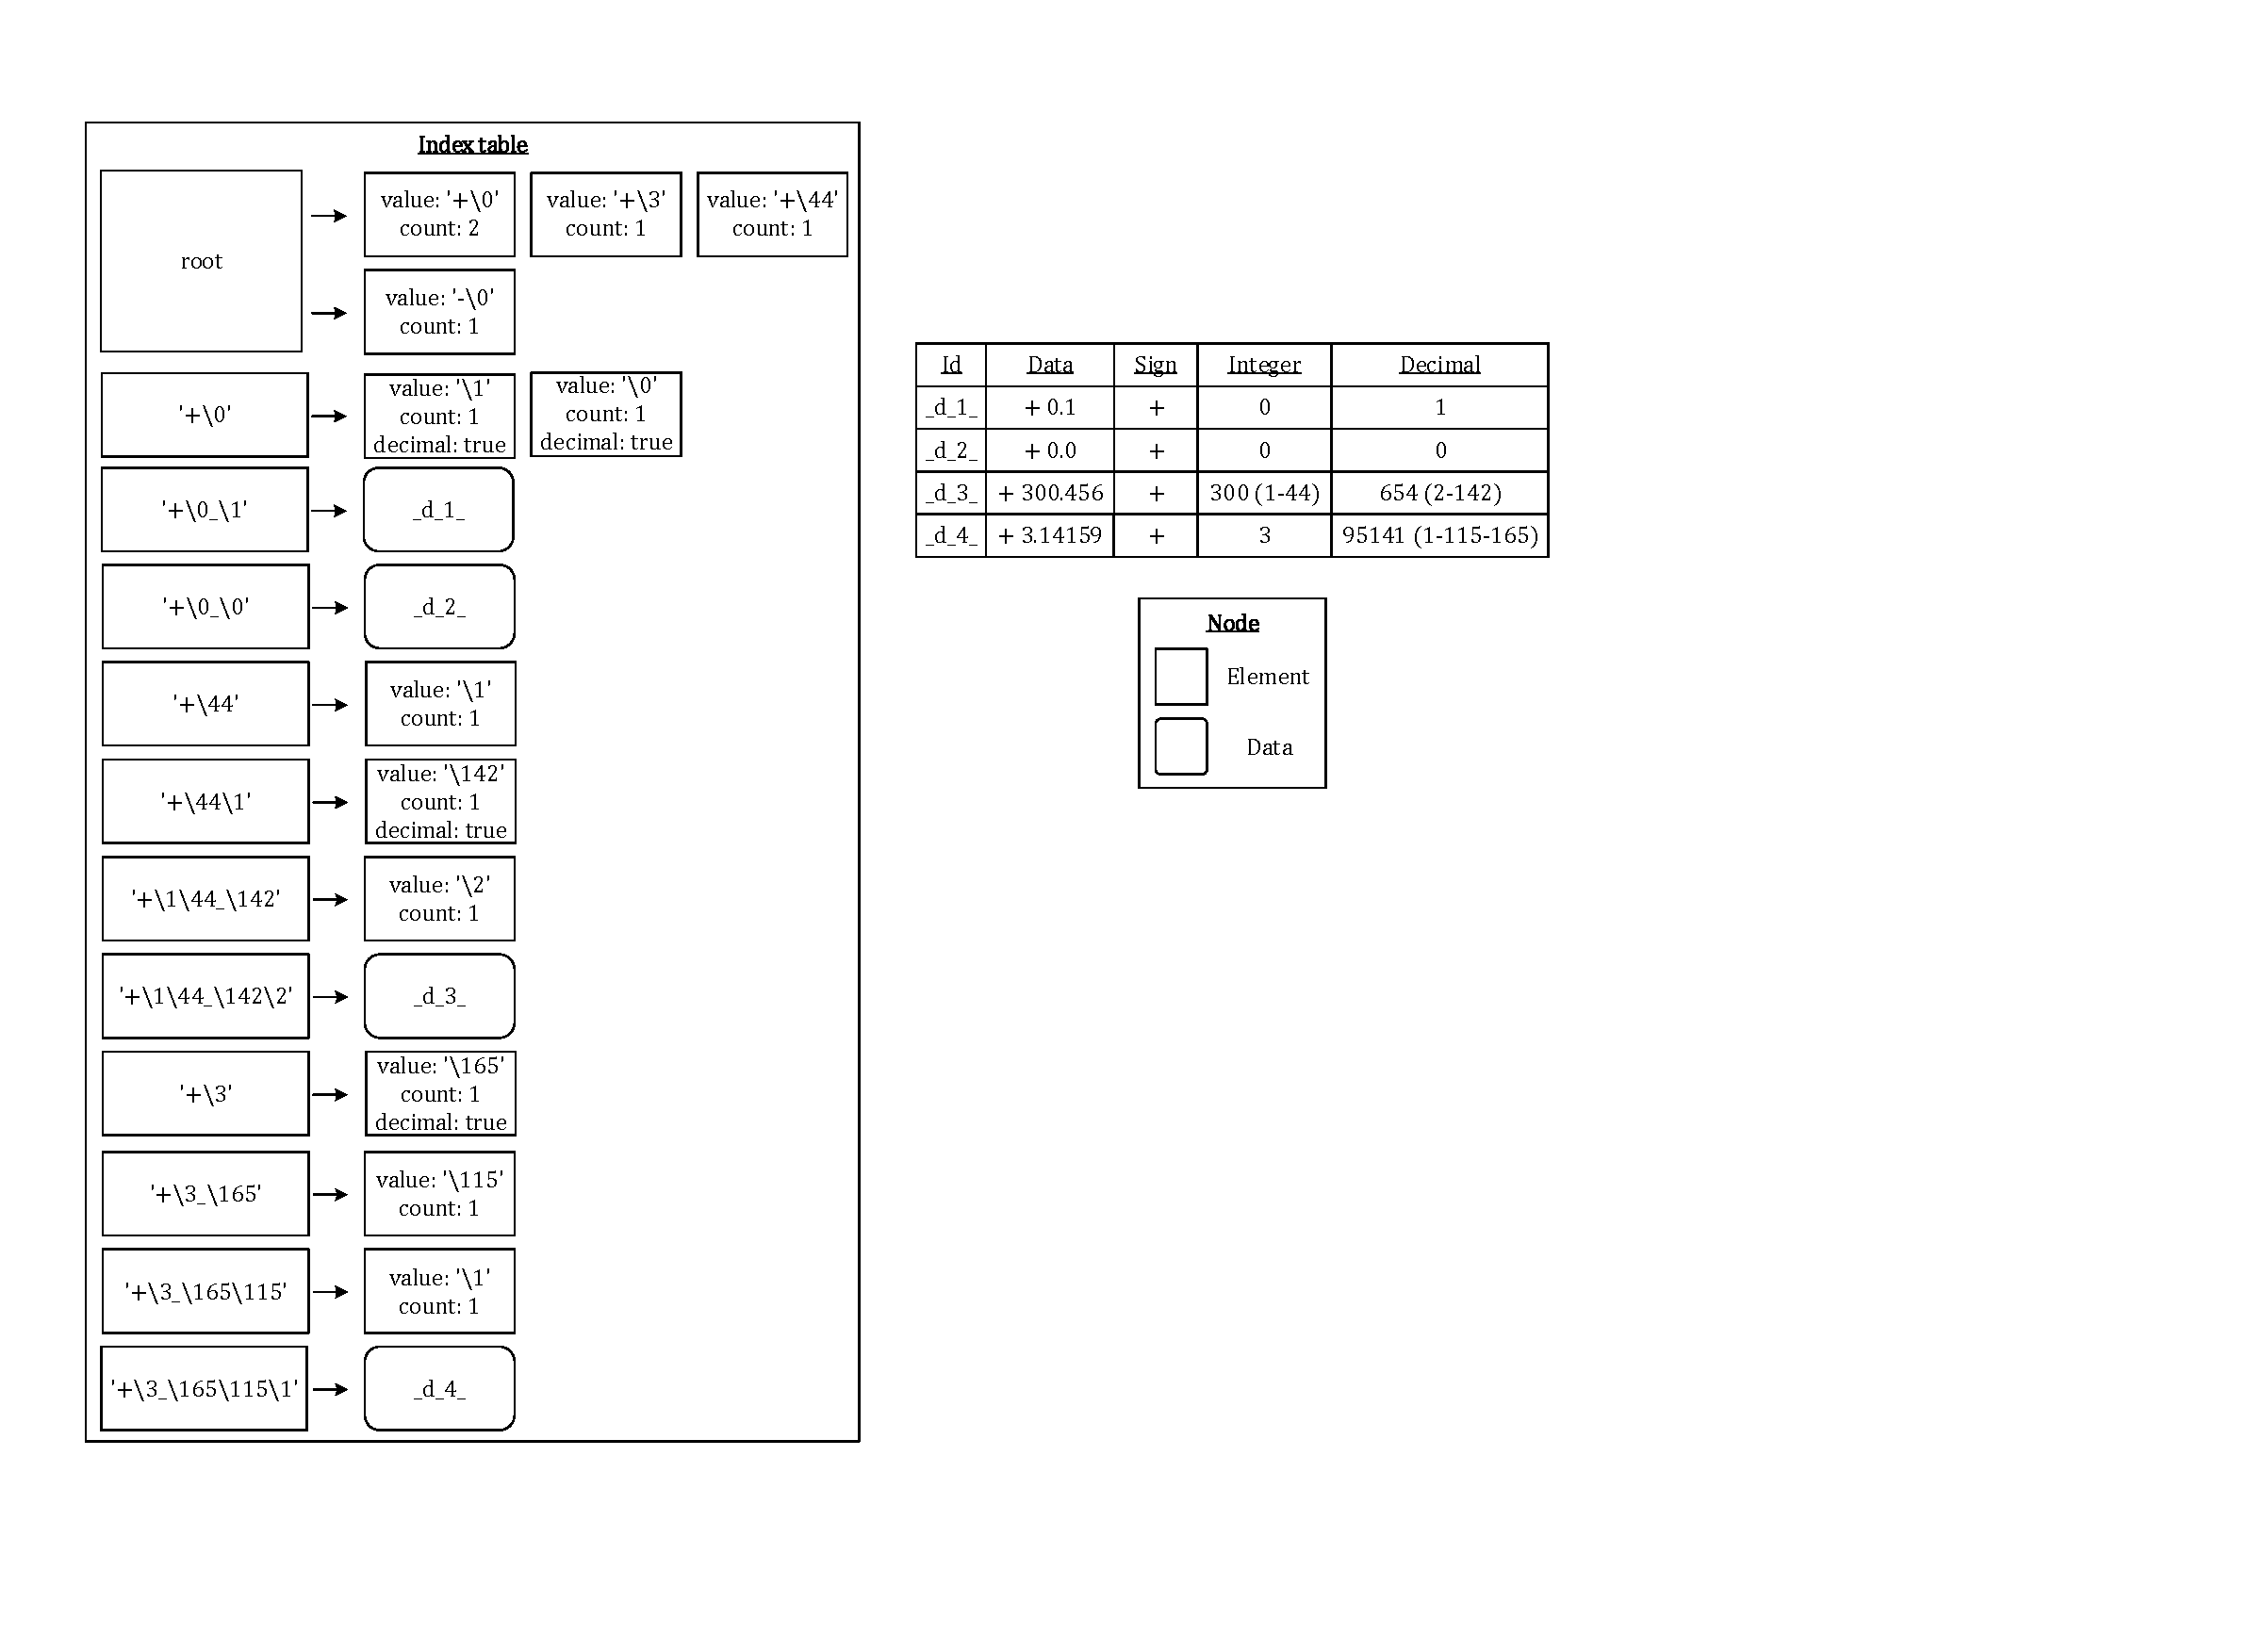
\includegraphics[width=0.8\textwidth]{./algorithm/real/pic/modification/example_v4.pdf}
\caption{The table after modified the value.}
\label{fig:algorithm:real:modification:example}
\end{figure}



% Selection section
\subsubsection{Selection}

The follow operations will use figure \ref{fig:algorithm:real:modification:example} as the example.

% Selection section enumerate
\begin{enumerate}

% --------------------------------------------------------

% Equal
\item \textbf{Equal}

If search \textit{0.0}, then convert it into three part: \textit{"Sign"}, \textit{"Integer"} and \textit{"Decimal"}, which means $'$+$\backslash0\backslash\_\backslash0'$ and use this as key to get the result, this should take $O(1)$.

% --------------------------------------------------------

% Not equal
\item \textbf{Not equal}

If searching the result which is not equal \textit{0.0}, strat of convert it into key, then start from root, then recursively to find the data nodes and only skip the key of input. This operation should take $O(b)$.

% --------------------------------------------------------

% Less than
\item \textbf{Less than}

When comparing the \emph{"Less than"} or \emph{"Greater}, the flow is way different as the other because of the dynamic byte design.

For example searching \textit{300.0} in table, then convert into string $'$+$\backslash44\backslash1\_\backslash0'$ which the length of \textit{"Integer"} is \textit{2} and \textit{1} for \textit{"Decimal"} that the two value is use to let the compare function know how deep of the byte need to search.

% Less than section enumerate
\begin{enumerate}

% Input value is a negative value
\item \textbf{Input value is a negative value}

\begin{enumerate}

\item Start from root and only get the nodes which the \textit{"Sign"} are \textit{'-'}.

\item When searching \textit{"Integer"} part, recursively to search the element node contain \textit{decimal} with the length is \textit{"longer than or equal to"} to the \textit{"Integer"} length of input (in this case is \textit{2}). Then only remain the nodes that the value of \textit{"Integer"} is \textit{"larger than or equal to"} the value in \textit{"Integer"} part of input.

\item Searching in \textit{"Decimal"} part:
\begin{enumerate}

\item If the length of \textit{"Integer"} part is \textit{"longer than"} the input, then get all the data nodes.

\item If the length of \textit{"Integer"} part is \textit{"equal to"} the input, then recursively and only get the element nodes that the length is \textit{"greater than or equal to"} the length of \textit{"Decimal"} of input. And check the value of \textit{"Decimal"} is \textit{"larger than"} the value in \textit{"Decimal"} part of input.
\end{enumerate}

\end{enumerate}

% Input value is a positive value
\item \textbf{Input value is a positive value}

\begin{enumerate}

\item Get all the data nodes start from root which the \textit{"Sign"} are \textit{'-'}.

\item Next start from root and get the nodes which the \textit{"Sign"} are \textit{'+'}.

\item When searching \textit{"Integer"} part, recursively to search the element node contain \textit{decimal} with the length is \textit{"shorter than or equal to"} to the \textit{"Integer"} length of input (in this case is \textit{2}). Then only remain the nodes that the value of \textit{"Integer"} is \textit{"smaller than or equal to"} than the value in \textit{"Integer"} part of input.

\item Searching in \textit{"Decimal"} part:
\begin{enumerate}

\item If the length of \textit{"Integer"} part is \textit{"shorter than"} the input, then get all the data nodes.

\item If the length of \textit{"Integer"} part is \textit{"equal to"} the input, then recursively and only get the element nodes that the length is \textit{"shorter than or equal to"} the length of \textit{"Decimal"} of input. And check the value of \textit{"Decimal"} is \textit{"smaller than"} the value in \textit{"Decimal"} part of input.
\end{enumerate}

\end{enumerate}

% Input value is equal to 0.0
\item \textbf{Input value is equal to \textit{0.0}}

Get all the data nodes start from root which the \textit{"Sign"} are \textit{'-'}.

% End Less than section enumerate
\end{enumerate}

The \emph{"Less than or equal to"} comparison is just do the \emph{"Less than"} and \emph{"Equal"} operation and then combine both result for ouput. The time complexity is $O(b)$ for both operation.

% --------------------------------------------------------

% Greater than
\item \textbf{Greater than}

This comparison flow is similar as \emph{"Less than"}.

% Greater than section enumerate
\begin{enumerate}

% Input value is a negative value
\item \textbf{Input value is a negative value}

\begin{enumerate}

\item Get all the data nodes start from root which the \textit{"Sign"} are \textit{'+'}.

\item Next start from root and get the nodes which the \textit{"Sign"} are \textit{'-'}.

\item When searching \textit{"Integer"} part, recursively to search the element node contain \textit{decimal} with the length is \textit{"shorter than or equal to"} to the \textit{"Integer"} length of input. Then only remain the nodes that the value of \textit{"Integer"} is \textit{"larger than or equal to"} than the value in \textit{"Integer"} part of input.

\item Searching in \textit{"Decimal"} part:
\begin{enumerate}

\item If the length of \textit{"Integer"} part is \textit{"shorter than"} the input, then get all the data nodes.

\item If the length of \textit{"Integer"} part is \textit{"equal to"} the input, then recursively and only get the element nodes that the length is \textit{"shorter than or equal to"} the length of \textit{"Decimal"} of input. And check the value of \textit{"Decimal"} is \textit{"larger than"} the value in \textit{"Decimal"} part of input.
\end{enumerate}

\end{enumerate}

% Input value is a positive value
\item \textbf{Input value is a positive value}

\begin{enumerate}

\item Start from root and only get the nodes which the \textit{"Sign"} are \textit{'+'}.

\item When searching \textit{"Integer"} part, recursively to search the element node contain \textit{decimal} with the length is \textit{"longer than or equal to"} to the \textit{"Integer"} length of input. Then only remain the nodes that the value of \textit{"Integer"} is \textit{"larger than or equal to"} the value in \textit{"Integer"} part of input.

\item Searching in \textit{"Decimal"} part:
\begin{enumerate}

\item If the length of \textit{"Integer"} part is \textit{"longer than"} the input, then get all the data nodes.

\item If the length of \textit{"Integer"} part is \textit{"equal to"} the input, then recursively and only get the element nodes that the length is \textit{"greater than or equal to"} the length of \textit{"Decimal"} of input. And check the value of \textit{"Decimal"} is \textit{"larger than"} the value in \textit{"Decimal"} part of input.
\end{enumerate}

\end{enumerate}

% Input value is equal to 0.0
\item \textbf{Input value is equal to \textit{0.0}}

Get all the data nodes start from root which the \textit{"Sign"} are \textit{'+'} but skip the key of \textit{+0.0}.

% End Greater than section enumerate
\end{enumerate}

The \emph{"Greater than or equal to"} comparison is just do the \emph{"Greater than"} and \emph{"Equal"} operation and then combine both result for ouput. The time complexity is $O(b)$ for both operation.

% --------------------------------------------------------

% Between
\item \textbf{Between}

The \textit{between} operation of \textit{REAL} is as same as the \textit{between} operation of the \textit{signed INTEGER}, so skip the description of this part. The time complexity is $O(b)$.

% --------------------------------------------------------

\end{enumerate}


% Summary section
\subsubsection{Summary}

Table \ref{table:algorithm:real:summary:time_complexity} is a summary the time complexity of each opration in \textit{REAL} type.

\begin{table}[h]
\centering
\caption{Time complexity for \textit{REAL} type.}
\label{table:algorithm:real:summary:time_complexity}
\begin{tabular}{|c|c|}

\hline
\multicolumn{1}{|c|}{Operation} &
\multicolumn{1}{c|}{\tabincell{c}{
Time complexity \\ ($b$: The byte length of data)
}} \\

\hline
\multicolumn{1}{|c|}{Insert} &
\multicolumn{1}{c|}{$O(b)$} \\

\hline
\multicolumn{1}{|c|}{Modify} &
\multicolumn{1}{c|}{$O(b)$} \\

\hline
\multicolumn{1}{|c|}{Delete} &
\multicolumn{1}{c|}{$O(b)$} \\

\hline
\multicolumn{1}{|c|}{Equal} &
\multicolumn{1}{c|}{$O(1)$} \\

\hline
\multicolumn{1}{|c|}{\tabincell{c}{Equal (muti-value)}} &
\multicolumn{1}{c|}{$O(1)$} \\

\hline
\multicolumn{1}{|c|}{Not equal} &
\multicolumn{1}{c|}{$O(b)$} \\

\hline
\multicolumn{1}{|c|}{\tabincell{c}{Not equal (muti-value)}} &
\multicolumn{1}{c|}{$O(b)$} \\

\hline
\multicolumn{1}{|c|}{Less than} &
\multicolumn{1}{c|}{$O(b)$} \\

\hline
\multicolumn{1}{|c|}{Less than or equal} &
\multicolumn{1}{c|}{$O(b)$} \\

\hline
\multicolumn{1}{|c|}{Greater than} &
\multicolumn{1}{c|}{$O(b)$} \\

\hline
\multicolumn{1}{|c|}{Greater than or equal} &
\multicolumn{1}{c|}{$O(b)$} \\

\hline
\multicolumn{1}{|c|}{Between} &
\multicolumn{1}{c|}{$O(b)$} \\

\hline
\end{tabular}
\end{table}

\textit{REAL} is target for the data type of \textit{"long double"}, the only disadvantage that it will need more byte to store the value compare with \textit{"long double"}. From table \ref{table:algorithm:real:design_data_type} shows that the \textit{"float"} can store the range beyond the \textit{"Bigint"}, so that this mean it will need many \textit{"Bigint"} to store the value in \textit{"long double"}.

\begin{table}[h]
\centering
\caption{Information about data type.}
\label{table:algorithm:real:design_data_type}
\begin{tabular}{|c|c|c|}

\hline
\multicolumn{1}{|c|}{Data type} &
\multicolumn{1}{c|}{Range} &
\multicolumn{1}{c|}{Bytes} \\

\hline
\multicolumn{1}{|c|}{float} &
\multicolumn{1}{c|}{$3.40282e^{+038}$ $\thicksim$ $1.17549e^{-038}$} &
\multicolumn{1}{c|}{4} \\

\hline
\multicolumn{1}{|c|}{double} &
\multicolumn{1}{c|}{$1.79769e^{+308}$ $\thicksim$ $2.22507e^{-308}$} &
\multicolumn{1}{c|}{8} \\

\hline
\multicolumn{1}{|c|}{long double} &
\multicolumn{1}{c|}{$1.18973e^{+4932}$ $\thicksim$ $3.3621e^{-4932}$} &
\multicolumn{1}{c|}{16} \\

\hline
\multicolumn{1}{|c|}{unsigned int} &
\multicolumn{1}{c|}{0 $\thicksim$ 4294697295} &
\multicolumn{1}{c|}{4} \\

\hline
\multicolumn{1}{|c|}{\tabincell{c}{
unsigned long long int \\ (Bigint)
}} &
\multicolumn{1}{c|}{0 $\thicksim$ 18446744073709551615} &
\multicolumn{1}{c|}{8} \\

\hline
\end{tabular}
\end{table}

But the advantage of \textit{REAL} that it can store the value with 100\% accuracy, also provide comparison and sorting, and it can store limitless data range. So no matter the basic use of the floating point such as Financial or Basic operations, these usage is hard to use more than five digital in \textit{"Decimal"} part. Also \textit{REAL} can store special data like science data such as the value in physics, this kind of usage may need to use up to thousand digital in \textit{"Decimal"} part, this is a normal range of \textit{"long double"}.\\



\clearpage

